% =====================================================================
%  PLCSP-DRL — 初稿
%  模板：Elsevier 标准双栏（elsarticle, 5p = two-column, 数字制引用）
%  编译：pdflatex -> bibtex -> pdflatex -> pdflatex
% =====================================================================
\documentclass[final,5p,times,twocolumn,number]{elsarticle}

\usepackage{amsmath,amssymb}
\usepackage{graphicx}
\usepackage{booktabs}
\usepackage{multirow}
\usepackage{threeparttable}
\usepackage{siunitx}
% hyperref：bbl 用 \href{...}{\path{doi:...}} 排 DOI，而 \path 由 hyperref 提供。
% 缺它时 bbl 会把 \path 退化成恒等宏，DOI 里的 "_" 就会触发数学模式报错。
\usepackage[hidelinks]{hyperref}
\usepackage{algorithm}
\usepackage{algpseudocode}
\usepackage{xcolor}

% ---- 图路径 ----
\graphicspath{{figures/}}

% ---- 浮动体（8 图 + 12 表 + 1 算法框）----
% ⚠️ 这里**不能放松**：`topfraction` 调到 0.9 以上会让 LaTeX 把浮动体
% 全推到章末连堆四页，正文与图表脱节。用接近默认的保守值，逼它插进正文。
\usepackage{placeins}          % 提供 \FloatBarrier
\setcounter{topnumber}{3}
\setcounter{bottomnumber}{2}
\setcounter{totalnumber}{5}
\renewcommand{\topfraction}{0.80}
\renewcommand{\bottomfraction}{0.60}
\renewcommand{\textfraction}{0.15}
\renewcommand{\floatpagefraction}{0.75}

% ---- 常用宏（只做缩写，不引入新概念；一律 \ensuremath 以便文本/数学两态通用）----
\newcommand{\Cmax}{\ensuremath{C_{\max}}}
\newcommand{\wj}{\ensuremath{w_j}}
\newcommand{\TWT}{\ensuremath{\mathrm{TWT}}}
\newcommand{\kWh}{\ensuremath{\mathrm{kWh}}}
\newcommand{\logp}{\ensuremath{\log \pi}}

\journal{Journal of Manufacturing Systems}

\begin{document}

\begin{frontmatter}

\title{Joint-chain group-relative reinforcement learning for
production--logistics collaborative scheduling}

\author[a]{Yuan Wang}
\author[a]{Naiming Xie\corref{cor1}}
\author[b]{Mingshan Li}

% TODO(投稿前): 通讯作者邮箱待填——本文件不代填。
\cortext[cor1]{Corresponding author.}

\address[a]{College of Economics and Management, Nanjing University of
Aeronautics and Astronautics, 29 Jiangjun Avenue, Nanjing, 211106, China}
\address[b]{Guangdong University of Petrochemical Technology, 139 Guanduer Rd,
Maoming, 525011, China}

\begin{abstract}
Production--logistics collaborative scheduling couples a flexible job shop
with a fleet of automated guided vehicles. We formulate the two layers as a
single decision chain and train it with group-relative policy optimization, so
that every production and logistics decision in an episode contributes to one
log-probability and one advantage. The policy is a standard Transformer over a
token sequence with a candidate-scoring head per decision kind, and ten
constraints are modelled as independent switches, each with a mechanism that
gives the policy something to act on. We measure the method on MK01 of the MKT
benchmark against a rule baseline, a single-objective version of itself, and
NSGA-II. On the fully constrained problem it dominates all twelve
out-of-sample points of the metaheuristic front; on the unconstrained problem
the metaheuristic is marginally ahead. Three further results are reported.
First, the aggregate energy consumption commonly reported in this literature is
close to rank-equivalent with the makespan, because the terms that dominate it
are linear in the horizon by construction, so energy adds a third dimension
only under a net account that removes those terms. Second, an ablation over the
advantage shows that subtracting a group-mean baseline has a measurable effect
while dividing by the group standard deviation does not. Third, a hypothesis
that single-objective ablation systematically misses mechanisms did not survive
its test.

\end{abstract}

\begin{keyword}
production--logistics collaborative scheduling \sep
flexible job shop scheduling \sep
automated guided vehicles \sep
reinforcement learning \sep
group-relative policy optimization \sep
multi-objective optimization
\end{keyword}

\end{frontmatter}

\section{Introduction}
\label{sec:intro}

A flexible job shop does not run on machines alone. Jobs must be moved between
machines, and in an automated shop that movement is performed by a fleet of
automated guided vehicles whose availability, routing, and load state determine
whether a machine that is ready to work has anything to work on. Deciding the
two layers separately, fixing the production plan first and dispatching vehicles
to execute it afterwards, is the conventional decomposition. It is exact only when
transport is never the limiting resource. In an automated shop it can be, and
the coupling is then exactly what the decomposition discards: the production
plan determines which transport tasks exist and when they are due, and the
dispatch decisions determine whether the machines are ever fed.

The integrated problem is known in the recent literature as the
production--logistics collaborative scheduling problem
(PLCSP)~\citep{li2025plcsp,shi2025nested}, and in an older line as integrated
scheduling of machines and AGVs~\citep{ulusoy1993}. Both lines are active
today. Reinforcement learning is the dominant recent tool, applied through a
variety of representations: multi-agent PPO over hand-built priority
vectors~\citep{li2025plcsp}, nested hierarchical
architectures~\citep{shi2025nested}, heterogeneous graph
attention~\citep{taagnet2026,yang2026hgamppo,yue2027hchgnn}, and hybrid
GNN--Transformer encoders~\citep{gao2026gnntransformer}. A parallel line
attacks the same coupling with hand-designed search such as large-neighbourhood
search and Benders decomposition, and solves closely related three-layer
problems well~\citep{chen2025carseq,chen2026benders}. The two lines differ in
what they cost to extend: the search-based methods are tailored per problem,
and a change to the constraints generally means redesigning the encoding or the
cuts, whereas a learned policy is in principle indifferent to which constraints
are switched on.

That second property is the reason this paper exists, and it is also why the
field's current state is worth examining closely. Across the recent work, the
architecture has converged while the constraint coverage has not. Congestion
and path conflict are excluded in at least eleven papers, three of which name
the cause rather than the choice: an encoder that carries only connectivity
cannot represent congestion, so a policy using it cannot learn to avoid
it~\citep{gao2026gnntransformer,taagnet2026,li2025plcsp}. Preventive
maintenance is listed as future work rather than modelled~\citep{zhang2026amr}.
Batching as a decision appears in warehouse order picking but not in transport
inside a job shop~\citep{wang2025gphh}. Charging is modelled in several
works~\citep{huang2025collaborative,dong2026handling}, but whether the
constraint ever activates under the parameters used is rarely reported.

Two consequences follow, and they set up the contribution. First, a model can
carry a constraint that never fires. A constraint that is modelled but never
violated, or modelled but never actionable, contributes nothing to the problem
and nothing to the comparison. Whether it fires is reported rarely, one
constraint at a time, and never --- in the work we surveyed --- for every
modelled constraint of a benchmark family at once; the closest case counts the
actions one constraint triggers, on a single
instance~\citep{huang2025collaborative}.
Section~\ref{sec:results:active} reports activation for all ten constraints
across the whole benchmark. Second, an architecture
claim and a constraint-handling claim are different claims, and the second is
where the field is uneven. Section~\ref{sec:related} documents both.

Figure~\ref{fig:motivation} shows the decomposition failing on a three-machine
shop, and what changes when the two layers are decided together.

\begin{figure*}[htbp]
\centering
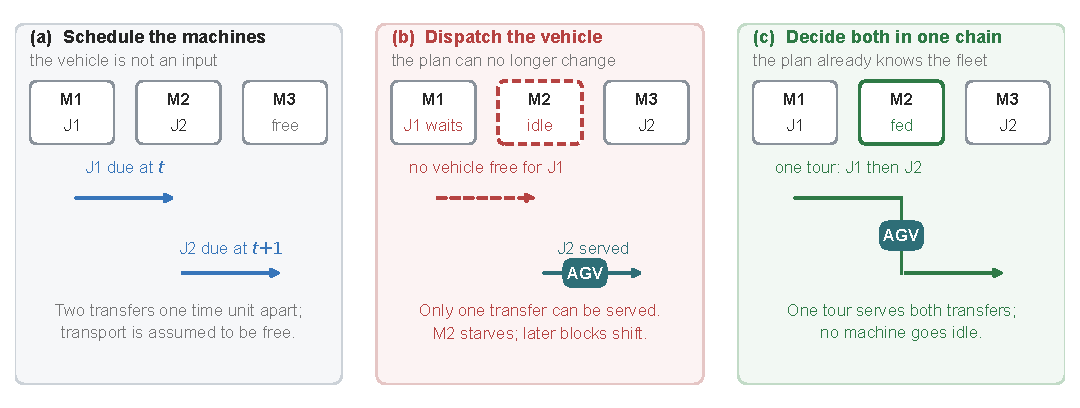
\includegraphics[width=\textwidth]{fig_motivation.pdf}
\caption{Deciding production and transport separately breaks down when the
vehicle fleet is the limiting resource; deciding them in one chain does not.
The shop has three machines and one vehicle. In (a) the machine schedule is
fixed first, with the vehicle absent from its input: it places two transfers
one time unit apart, job $J_1$ from $M_1$ to $M_2$ and job $J_2$ from $M_2$ to
$M_3$, because it assumes that transport is always available. In (b) the
vehicle is dispatched to execute that plan, and one vehicle cannot serve both
transfers: $J_1$ waits while the vehicle carries $J_2$, $M_2$ has nothing to
work on, and every later block on that machine shifts, so the loss appears as
idle machine time rather than as a worse machine sequence. In (c) both layers
are decided in one chain, so the plan is built knowing what the fleet can
deliver, and a single tour serves $J_1$ and then $J_2$ without idling any
machine. The example is constructed to make the mechanism visible and is not
drawn from a measured run.}
\label{fig:motivation}
\end{figure*}

This paper therefore spends its effort on the constraints and on the
representation they need. The policy's parts are standard: a Transformer
encoder, a candidate-scoring head per decision kind, and group-relative policy
optimization. What the paper adds to them is a formulation and a
representation. The formulation is the joint chain, which carries every
production and logistics decision of an episode under one log-probability and
one advantage. The representation is the transport-network-aware encoding of
Section~\ref{sec:method:state}, which puts the aisle network into the state
rather than leaving it to be inferred from the machine and vehicle tokens.
Every constraint then gets a mechanism that gives the policy something to act
on: a decision point where a rule used to decide, a dynamics change where the
model was incomplete, or an input feature where the state was not visible.
Every switch defaults to off with bit-identical behaviour, so that an ablation
measures the mechanism and not an incidental change elsewhere.
Section~\ref{sec:related:coverage} sets out, for each of the ten constraints,
what prior work does and what this paper does.

\paragraph{What we find}

On the fully constrained problem the learned policy dominates every
out-of-sample point of an NSGA-II front: the front's best re-evaluated values
are 79.56 for makespan, 6.239 for energy, and 20.73 for tardiness, against
78.90, 6.160, and 5.042 for the policy, and all twelve front points are
dominated. On the unconstrained problem the ordering reverses and NSGA-II edges
ahead, 49.14 against 49.27, on a problem where it has five thousand
deterministic evaluations available. That pair of results locates the method's
advantage in its representation of the constrained state rather than in its
search behaviour, which is the claim the rest of the paper examines.

Two further observations are worth stating before the results. An ablation over
the advantage shows that subtracting a group-mean baseline does measurable work
while dividing by the group standard deviation does not, which is a narrower
statement than the one usually made about group-relative advantages. And a
hypothesis we set out to confirm (that ablating on the makespan alone
systematically misses mechanisms) did not survive its own test. One property of
the reported objectives is not an observation at all and is stated where the
results are given: the energy account cannot move independently of the
makespan, because most of it is tied to the horizon by definition
(Section~\ref{sec:results:energy}).

\paragraph{Contributions}

\begin{enumerate}
\item \textbf{A joint-chain formulation, and a measurement of which part of it
      matters.} Production and logistics decisions in one episode are treated
      as one decision chain with one log-probability and one group-relative
      advantage, rather than as separate agents. We give the reason (group
      relative advantage compares samples within a group, and a group drawn
      from two policies is not a group) and then measure it. The
      measured answer is narrower than the usual statement: subtracting the
      group mean matters, dividing by the group standard deviation does not
      (Section~\ref{sec:results:advantage}). The arrangement is not merely a
      convenience: a recent comparison of joint and modular training on a job
      shop with transport resources finds a coordination gap, in which the
      modular arrangement does not recover what joint training
      obtains~\citep{link2026coordination}.

\item \textbf{A transport-network-aware encoding, and a mechanism for each of
      ten constraints.} The encoders in this literature carry the network's
      structure but not its live state: three papers state that theirs cannot
      represent congestion, so a policy using one cannot learn to avoid it.
      Where the network does enter an encoder it enters as static topology. We
      therefore make the transport network itself part of the state. The
      aisle segments become tokens carrying their own occupancy, a
      distance-dependent bias enters the attention score, and the route head
      reads the segments each candidate traverses. The aisle stops
      being something the policy is told about and becomes something it can act
      on. The remaining mechanisms follow the same discipline: a decision point
      where a rule used to decide, a dynamics change where the model was
      incomplete, or an input feature where the state was not visible.
      Section~\ref{sec:related:coverage} sets out the ten cases one by one and
      separates the ones where the difference is categorical from the ones where
      it is a matter of degree. Every switch defaults to off and reproduces the
      pre-mechanism trajectory bit for bit, which is what makes the ablations
      measurements rather than comparisons against an unstated baseline. We do
      not claim that the encoding transfers to shop layouts it was not trained
      on; the mechanisms are demonstrated on the layout of the instance.

\item \textbf{Results reported against interest.} We report the ablation table
      as a grouping rather than as an ordering, because the measured
      training-seed standard deviation is the same order as most of the
      differences in it. We report the hypothesis about single-objective
      ablation that did not hold, and the constraints that do not activate
      under the reported parameters, so that the coverage claim is a statement
      about the model rather than about demonstrated effects.
\end{enumerate}

\paragraph{Scope} The evaluation in this paper is a first pass. It uses one
instance of the MKT benchmark and a single training run per configuration, with
five seeds per arm reserved for the advantage ablation because that comparison
is about the training procedure itself. Section~\ref{sec:discussion} states
what this bounds. The experimental protocol is designed so that widening it
later changes the tables rather than the claims.

The remainder of the paper is organized as follows.
Section~\ref{sec:related} reviews the two literature lines, sets out the
constraint-by-constraint coverage, and explains why published figures from this
literature are not reproduced in our tables. Section~\ref{sec:problem}
formulates the problem, the ten constraints, and the three objectives.
Section~\ref{sec:method} describes the policy, the training procedure, and the
mechanism for each constraint. Section~\ref{sec:setup} gives the benchmark, the
configuration, and the reproducibility discipline.
Section~\ref{sec:results} reports the results, including the one negative one.
Section~\ref{sec:discussion} states the limitations, and
Section~\ref{sec:conclusion} concludes.

\section{Related work}
\label{sec:related}

\subsection{Integrated scheduling of machines and vehicles}
\label{sec:related:plcsp}

Treating machine scheduling and vehicle dispatching as one problem has a
lineage that predates its current name. Ulusoy and
Bilge~\citep{ulusoy1993} scheduled machines and AGVs simultaneously and
proposed a genetic algorithm for the combined problem. The recent literature
has converged on the name production--logistics collaborative scheduling, used
by Li et al.~\citep{li2025plcsp} and Shi et al.~\citep{shi2025nested} among
others. The two names describe the same two-layer structure: a flexible job
shop decides which machine processes each operation, and a vehicle fleet
decides which vehicle performs each transfer.

The scope of the two layers is consistent across this literature, and so is one
boundary: reinforcement learning is used to control task allocation, that is
the assignment of operations to machines and of transfers to vehicles, while
local collision avoidance at the millisecond scale is delegated to the fleet
control system. We adopt the same boundary.

The problem also has an exact-optimisation line. Yao et al.~\citep{yao2026cp}
formulate the integrated problem as a constraint program and report that it
remains computationally intensive on the harder instances, which is the usual
motivation for learning-based approaches. The two lines are complementary
rather than competing.

Within the learning line, the decomposition varies. Hierarchical schemes
separate a high-level dispatching policy from lower-level execution, either as
a nested architecture~\citep{shi2025nested} or as an explicit layer
stack~\citep{wang2025hierarchical}; Wang et al.~\citep{wang2025hierarchical}
note that this design leans on the quality of the initial heuristic guidance
and can converge prematurely when that guidance is biased. Flat schemes place
all decisions in one policy, as Li et al.~\citep{li2025tsmc} do with a
multi-agent formulation over tasks, machines, and vehicles. Our formulation is
of the flat kind, and Section~\ref{sec:method:chain} gives the reason.

The set of resources being co-scheduled also varies. Yuan et
al.~\citep{yuan2026workers} schedule workers alongside AGVs in a distributed
flexible job shop, so that two heterogeneous transport resources compete for
the same jobs. We keep the resource set at machines and vehicles, which is the
boundary the PLCSP literature uses, and treat the wider resource set as out of
scope.

Whether the two layers are learned together or apart has itself become a
question. Link et al.~\citep{link2026coordination} compare joint and modular
training for a job shop with transport resources and find a coordination gap:
the modular arrangement does not recover what joint training obtains. That is
the closest published statement of the argument we make in
Section~\ref{sec:method:chain}, and it is about the training arrangement rather
than the architecture. Dong et al.~\citep{dong2026handling} reach the same
coupling from the exact-solution side, scheduling production together with
material-handling robots and carrying the robot battery state as an explicit
constraint. Dong et al.~\citep{dong2025heuristic} take the learning route on a
similar problem, with a heuristic supplying the dispatch decisions the policy
does not make.

\paragraph{Exact and metaheuristic treatments of the same coupling.}
A parallel line attacks the same production--logistics coupling with
hand-designed search rather than with a learned policy, and two of its members
are close enough to this paper to be worth stating precisely.
Chen et al.~\citep{chen2025carseq} integrate car sequencing on a mixed-model
assembly line with multi-trip vehicle routing and synchronized part supply; the
production sequence determines the due dates of the parts, which in turn
determine how the vehicles must be scheduled. That is the same asymmetric
causal chain we describe in Section~\ref{sec:method:chain}, in which production
creates the transport demand and fixes its deadlines. It is solved there
by a multi-start adaptive large-neighbourhood search with variable-neighbourhood
descent. Chen et al.~\citep{chen2026benders} couple order acceptance,
two-dimensional packing, and parallel machine scheduling, three decision layers
at once, and solve them by a nested logic-based Benders decomposition. Xu and
Xie~\citep{xu2025forest} couple scheduling with route planning in an emergency
setting, where the two layers also cannot be separated.

The methods in this line are problem-specific: an encoding, a decomposition, or
a set of cuts is designed per problem, and a change to the constraints
generally requires redesigning them. The same is true of the related machine
scheduling work in this line, where the algorithm is tailored to a
problem variant rather than transferred across
variants~\citep{chen2026upms}. The present work asks the complementary
question, whether a single learned policy over a state representation can serve
this class of coupled problems without per-problem algorithm design. We do not
claim that a learned policy beats these methods on the problems they were built
for; Section~\ref{sec:related:incomparable} explains why that comparison is not
available here, and Section~\ref{sec:results} reports where our policy does and
does not hold up against a metaheuristic on its own configuration.

\subsection{Learning architectures}
\label{sec:related:arch}

The dominant representation in recent work is a heterogeneous graph.
Xu et al.~\citep{taagnet2026} encode jobs, machines, and vehicles as three node
types with graph attention and type-aware pooling. Yang et
al.~\citep{yang2026hgamppo} combine heterogeneous graph attention with
multi-policy PPO. Yue et al.~\citep{yue2027hchgnn} build a hub-centric graph
for vehicle dispatching under finite-buffer constraints. Zhu et
al.~\citep{zhu2026dfjspht} apply a graph neural network to a distributed
flexible job shop with heterogeneous transport resources. Wu et
al.~\citep{wu2026madappo} use a heterogeneous graph attention network with
multi-head attention inside a two-agent PPO, for machine failures without
transport. Geng et al.~\citep{geng2025dtdrl} drive a multi-agent PPO from a
digital twin of the workshop, so the state is refreshed from a simulated copy
of the plant rather than from the shop itself.

A second line uses simpler sequence models. Li et al.~\citep{li2025plcsp} use a
multi-agent PPO with fully connected networks of 128-64-64 units and resolve
the final choice through a hand-written priority vector. Zhang et
al.~\citep{zhang2025sgformer} replace the graph encoder with a single-layer
simplified graph transformer to reach larger instances. Gao et
al.~\citep{gao2026gnntransformer} combine a graph convolutional stack with a
Transformer over task sequences. Wang et
al.~\citep{wang2025multitarget} train one policy to serve several scheduling
targets end to end, rather than one policy per target.

Our encoder is a standard Transformer~\citep{vaswani2017} over a token sequence
with no attention mask, and the novelty in this paper is not in the attention
mechanism. It is in what the attention is given to read, which is the token set
of Section~\ref{sec:method:state} and the transport-network-aware segment of
it. We note that the encoder choice is not a regression: recent work has moved
toward simplified representations and away from problem-specific graph
structure. Xiao et al.~\citep{xiao2026resched} reduce the flexible job shop to a
handful of state features behind a standard Transformer, and report that the
simplification does not cost performance; Wang et al.~\citep{wang2025memory} and
Zhang et al.~\citep{zhang2024improvement} keep a learned model in the loop but
use it to guide an improvement heuristic rather than to construct a schedule in
one pass. A plain attention encoder over a well-chosen token set sits within
that direction rather than against it.

Two further lines bear on how a policy is trained rather than what it reads.
Self-supervision can replace the reward signal entirely for job shop
scheduling~\citep{corsini2024selflabeling}, and a policy can be asked to serve
several preferences at once with self-evolution~\citep{choi2025multipolicy} or
to adapt per instance~\citep{qing2026instancewise}. Luttmann and
Xie~\citep{luttmann2026multiagentself} treat a set of simultaneous actions as
the object to improve, which is the closest formulation to our joint chain that
we have found outside this problem class. Stochastic processing times enter the
state through an attention encoder in~\citep{smit2025stochastic}. On the
application side, Zhu et al.~\citep{zhu2025matrix} couple the shop layout
itself to the scheduling policy, and Lee et
al.~\citep{lee2026digitaltwin} drive a dynamic AGV system from a digital twin.

What the representation must carry, however, is a substantive question and not
a matter of taste. Gao et al.~\citep{gao2026gnntransformer} state that their
encoder captures the static topology of the road network and therefore cannot
detect congestion arising from multi-vehicle interaction. Xu et
al.~\citep{taagnet2026} give vehicle features that contain neither coordinates
nor distances, so distance enters only through two hand-written dispatch rules.
Li et al.~\citep{li2025plcsp} use a network with no attention or graph
structure at all. In each case the constraint is absent from the state space,
and a policy cannot act on what its representation does not contain. The
mechanisms in Section~\ref{sec:method} that add aisle-segment tokens and a
distance bias to the attention score exist for this reason.

\subsection{Constraints and objectives}
\label{sec:related:constraints}

The constraints modelled in this literature vary, and the variation is
informative. Shi et al.~\citep{shi2025nested} state that machine breakdowns,
path conflicts, and AGV charging are ignored. Li et al.~\citep{li2025jms} state
that AGV failure is not considered and that time consumed by charging and
collision avoidance is negligible. Tang et
al.~\citep{tang2025lotstreaming} study static scheduling and do not consider
path conflict during travel. Wu et al.~\citep{wu2026madappo} state that energy
consumption is not involved and that workpieces and machines are all ready at
time zero, so transport does not enter. Zhang et
al.~\citep{zhang2026amr} treat maintenance of a deteriorating resource as
future work. Zhu et al.~\citep{zhu2026dfjspht} exclude transport route
conflicts and power replenishment. Yi et al.~\citep{yi2026petri} train without
accounting for AGV recharging needs. Li et al.~\citep{li2025plcsp} list AGV
charging, collision-avoidance-induced transport uncertainty, machine breakdown,
and worker absence as future work, and note that a DRL algorithm trained on one
workshop configuration needs retraining when the configuration changes.
Section~\ref{sec:related:coverage} revisits the same exclusions constraint by
constraint.



Charging is the exception to that pattern: papers do model battery state and
act on it, through a learned charging action~\citep{huang2025collaborative} or
a closed-form optimal rule~\citep{dong2026handling}, so a
claim that charging is unaddressed would be false. What is less often reported
is whether the constraint is ever active under the parameter values used:
whether a vehicle ever reaches the point where the decision matters.
Section~\ref{sec:results:active} measures that for our configuration, and finds
that it does not.

On objectives, the recent literature is predominantly makespan-first, with
energy entering either as a second objective or as a modelling contribution.
Yuan et al.~\citep{yuan2025green} build a five-component energy model with
multiple spindle speeds; Cheng et al.~\citep{cheng2025energy} combine deep
reinforcement learning with a memetic algorithm for an energy-saving variant.
Energy as a second objective also appears in the batch-processing line, where
Zheng et al.~\citep{zheng2025biobjective} solve a bi-objective non-identical
batch machine problem with makespan and energy exactly, and the batch
scheduling literature more generally is concerned with how batches are formed
and formulated~\citep{zheng2025formulations,xu2026autoclave,ding2024molding}. Energy is thus an established
objective, and the energy parameters we use are taken from Yuan et
al.~\citep{yuan2025green}. Multi-objective formulations appear in various
forms: a weighted sum over makespan and logistics
cost~\citep{shi2025nested}, and a Pareto-based hybrid that places a
non-dominated sorting step inside a DQN loop~\citep{tang2025lotstreaming}.

What we have not found in this line is a check on whether the reported
objectives are in fact independent of one another.
Section~\ref{sec:results:energy} runs that check. Preference conditioning is
the other current answer to the same problem: Smit et
al.~\citep{smit2026dcan} train a single policy over a preference vector and
recover a whole front from it, which is the natural extension of what this
paper reports for a fixed weight vector.

Maintenance is treated separately. Decisions about when to maintain or replace
a deteriorating system are studied in the reliability literature, where the
decision variable is a replacement or ordering policy rather than a scheduling
action~\citep{dong2024orderreplacement,dong2025sparepart}. Our maintenance
mechanism is of the scheduling kind (the policy chooses when to take an idle
machine out of service, within a forced threshold), and we are not aware of a
scheduling formulation of that decision in this problem class.

\subsection{How the ten constraints have been handled}
\label{sec:related:coverage}

Constraint coverage is set out below. The separation that matters is between a
constraint prior work does not handle and one it handles differently: not
having done something is weak evidence, whereas a treatment that differs in a
way that changes what the policy can do is a claim of substance.

\begin{description}\itemsep3pt
\item \textbf{C1 --- congestion.} \emph{Prior work.} Eleven works in this line exclude
      congestion or list it as future work. Three of them name the cause: the
      encoder carries only static topology, so ``the model cannot detect or
      avoid congestion that emerges in real time from multi-AGV
      interactions''~\citep{gao2026gnntransformer}; the vehicle features contain
      neither coordinates nor distances~\citep{taagnet2026}, and distance enters
      only through hand-written dispatch rules; and one policy network has no
      attention or graph structure at all~\citep{li2025plcsp}. Four works do
      choose a route, but leave congestion awareness to the simulator or to a
      rule. \emph{This paper.} The transport network enters the state: the aisle
      segments become tokens, a distance bias enters the attention score, and
      the route head reads the segments its candidate traverses
      (Section~\ref{sec:method:state}). \emph{Relation.} Not handled, with the
      cause stated by the authors. This is the strongest form of the claim
      available here, because it is a statement about the representation rather
      than about effort.
\item \textbf{C2 --- finite buffers.} \emph{Prior work.} Finite output buffers with a
      deadlock-aware priority mask that blocks all dispatching while any buffer
      holds a finished part~\citep{yue2027hchgnn}; others assume infinite
      capacity~\citep{taagnet2026,li2025plcsp}. \emph{This paper.} Buffer
      occupancy is a machine-token feature, and the constraint is otherwise left
      to the budget mechanism. \emph{Relation.} Handled differently: a
      hand-written mask versus a learned policy over the same state.
\item \textbf{C3 --- machine failure.} \emph{Prior work.} Memoryless failure at a fixed
      rate, and in several studies a single fixed failure scenario rather than
      a sampled process~\citep{wu2026madappo,geng2025dtdrl}. \emph{This paper.}
      The failure rate rises with the maintenance clock along a Weibull hazard.
      \emph{Relation.} Age dependence is not handled elsewhere. The rate law and
      its shape parameter are assumed, not calibrated to plant data.
\item \textbf{C4 --- rework.} \emph{Prior work.} A reworked operation returns to the task
      pool and is reassigned to a machine and a vehicle~\citep{li2025tsmc}.
      \emph{This paper.} Rework is performed in place on the same machine, as
      the simulation defines it, so no decision point is introduced.
      \emph{Relation.} Handled differently, by a modelling choice rather than by
      a mechanism.
\item \textbf{C5 --- setup.} \emph{Prior work.} Sequence-dependent setup as a
      machine--job edge attribute in the graph, with a shortest-setup-time
      baseline~\citep{yue2027hchgnn}; explicit setup tables in the general
      job-shop setting. Others assume immediate setup~\citep{taagnet2026}.
      \emph{This paper.} The setup time of a job change is a property of the
      pair rather than of either entity, so it is supplied to the machine head
      as a candidate feature. \emph{Relation.} Handled differently. Setup is the
      largest lever in our ablation (Table~\ref{tab:ablation}), so the treatment
      is consequential.
\item \textbf{C6 --- due dates.} \emph{Prior work.} Work-content due dates of the TWK
      family, with a per-job factor and an arrival term~\citep{taagnet2026,li2025plcsp};
      one work treats tardiness as a constraint rather than an
      objective~\citep{li2025plcsp}. \emph{This paper.} Due dates are exogenous,
      per job, and anchored on a load lower bound, so they do not move when the
      fleet configuration changes (Table~\ref{tab:duedates}). \emph{Relation.}
      Handled differently; exogeneity with respect to the fleet is the point of
      the design.
\item \textbf{C7 --- vehicle failure.} \emph{Prior work.} A failed vehicle releases its
      current task to the task pool and returns after
      repair~\citep{li2025plcsp}; three failure scenarios distinguished by when
      the failure occurs~\citep{shi2025nested}. \emph{This paper.} Tasks held by
      a failed vehicle are handed to vehicles that are still running, at
      checkpoints where the vehicle holds no aisle lock. \emph{Relation.}
      Handled differently: hand-over rather than return to a shared pool, with
      the target chosen by a rule rather than by the policy.
\item \textbf{C8 --- fleet and batching.} \emph{Prior work.} Vehicle capacity appears as
      a model parameter in five works, and none of them lets the policy decide
      how many tasks a trip should combine. Batching is a decision elsewhere,
      but a different one: in warehouse order batching the decision is which
      orders to pick together, coupled to the picker route rather than to a
      vehicle fleet~\citep{wang2025gphh}. We therefore do not claim that
      batching as a decision is new, only that transport batching inside a job
      shop is not where that decision has been studied. \emph{This paper.}
      Capacity is operational: one trip collects every queued task at a
      pick-up point and delivers to several drop points, and a separate head
      decides how many further tasks to append. \emph{Relation.} Handled
      differently, and the room the benchmark leaves for it is small
      (Table~\ref{tab:batching}).
\item \textbf{C9 --- charging.} \emph{Prior work.} Charging as a learned action over
      no-charge, opportunity-charge, and full-charge, with charger selection, on
      the same benchmark families~\citep{huang2025collaborative}; a closed-form
      optimal charging rule for a single-station variant~\citep{dong2026handling}.
      \emph{This paper.} A head chooses between not charging and each station
      when a vehicle is idle, and a vehicle at zero battery becomes unavailable
      until it recovers. \emph{Relation.} Handled differently, and not
      evaluated here: the constraint does not activate under the reported
      parameters (Table~\ref{tab:active}), so no claim is made about it.
\item \textbf{C10 --- maintenance.} \emph{Prior work.} No work in this line makes
      maintenance a decision. Four works list it as future work, and one models
      equipment deterioration while leaving the maintenance action
      open~\citep{zhang2026amr}. \emph{This paper.} A head chooses between
      starting maintenance on an idle machine now and deferring it, with the
      forced threshold as a hard floor. \emph{Relation.} Not handled elsewhere,
      but the constraint does not activate on the instance used for the policy
      results either, so the mechanism carries no measured effect here.
\end{description}

Two readings of this list are worth separating. The coverage claim itself: two
constraints are handled here as policy decisions that no surveyed work handles
that way, batch size and maintenance, and for congestion prior work not
only omits the constraint but states why its representation cannot carry it.
That last case is the substantive one, because it identifies a cause rather
than an omission.

The second reading is less comfortable. A constraint that no one has handled is
not automatically a contribution, and a constraint handled differently is a
difference rather than a novelty unless the difference changes what the policy
can do. For C2, C4, C5, C6, and C7 our treatment differs in where the
information enters, whether a candidate feature, a token, or a mask equivalent, and
these are differences of degree. For C8 and C10 the difference is categorical,
but the mechanisms carry no measured effect on the instance used here, so the
coverage is a statement about the model rather than about a demonstrated
result. What the list supports is that the model carries these constraints and
that the policy can act on them, not that each action improves the outcome.

\subsection{Where the field is moving}
\label{sec:related:landscape}

Four directions are visible in the most recent work on this problem, and our
design choices sit differently against each of them.

The heterogeneous graph with an attention encoder and a multi-policy PPO
backbone has become the default: it is the shared structure of the works by
Xu et al.~\citep{taagnet2026}, Yang et al.~\citep{yang2026hgamppo}, and Yue et
al.~\citep{yue2027hchgnn}. We depart from it in the encoder, for the
representation reasons given in Section~\ref{sec:related:arch}, and we keep the
single-policy structure for the advantage reasons given in
Section~\ref{sec:method:chain}.

Constraint realism is increasing. Finite buffers and deadlock, charging,
multi-trip load limits, deteriorating equipment, and worker availability now
appear individually in various papers~\citep{yue2027hchgnn,zhang2026amr,yuan2026workers}.
What is less common is a paper that carries many of them at once and reports
which of them are active. That is the gap this paper addresses, and
Section~\ref{sec:results:active} is the measurement.

Finally, the evaluation standard is rising. Recent work reports multiple
instance scales and, increasingly, real production data. Three current
benchmarks make the point: ATLAS draws on production traces from a large
manufacturing operator~\citep{jiang2026atlas}, DynaSchedBench calibrates
dynamic instances by difficulty and reports what it calls an observability
paradox in learned schedulers~\citep{cao2026dynaschedbench}, and FrontierCO
evaluates solvers at a scale that rules of thumb do not
reach~\citep{feng2026frontierco}. Our evaluation is the weakest part of this
paper by that standard, and Section~\ref{sec:discussion} takes it up.

\section{Problem formulation}
\label{sec:problem}

\subsection{Production and logistics}
\label{sec:problem:model}

We study the production--logistics collaborative scheduling problem (PLCSP).
The problem couples two decision layers that are usually solved apart:
a flexible job shop, where each operation must be assigned to one eligible
machine, and a fleet of automated guided vehicles (AGVs),
which must move every job between machines and to and from a load--unload
station. Assigning an operation to a machine is a decision; the order in which
a machine works through the jobs waiting at it is not one, and follows the
order in which the vehicles deliver them. The term follows the recent
literature on production--logistics
collaborative scheduling; the same problem class appears in the older
literature as integrated scheduling of machines and AGVs.

Let $\mathcal{J}$ be the set of $n$ jobs, $\mathcal{M}$ the set of $m$
machines, and $\mathcal{V}$ the set of $V$ vehicles. Job $j$ consists of
$n_j$ operations that must be processed in the fixed order
$O_{j,1} \to O_{j,2} \to \dots \to O_{j,n_j}$. Operation $O_{j,k}$ may be
processed on any machine in the eligible set $\mathcal{M}_{j,k} \subseteq
\mathcal{M}$; its processing time on machine $i$ is $p_{jki}$. If job
$j'$ is scheduled on a machine immediately after job $j$, a sequence-dependent
setup time $s_{jj'}$ elapses before $j'$ can start.

\paragraph{Shop layout and transport}
Machines occupy the cells of a two-dimensional grid with $n_{\mathrm{col}} =
\lceil \sqrt{m} \rceil$ columns and $n_{\mathrm{row}} = \lceil m /
n_{\mathrm{col}} \rceil$ rows. Empty cells are permitted. The aisles are the
grid lines between cells, so a passage never crosses a machine. The aisle
network is a graph whose nodes are the $(n_{\mathrm{row}}+1)(n_{\mathrm{col}}+1)$
intersections and whose edges are the horizontal and vertical segments between
adjacent intersections; the weight of an edge is its physical length. Each
machine has a dock, connected to the nearest corner intersection of its cell.
The load--unload (LU) station is a node outside the grid, joined to the left
boundary by one connecting segment. Jobs enter the shop at the LU station and
return there when their last operation is complete. Completion times are
therefore measured at the LU station, so the makespan of a job includes both
its entry travel and its return travel. Figure~\ref{fig:layout} shows the
layout.

\begin{figure}[htbp]
\centering
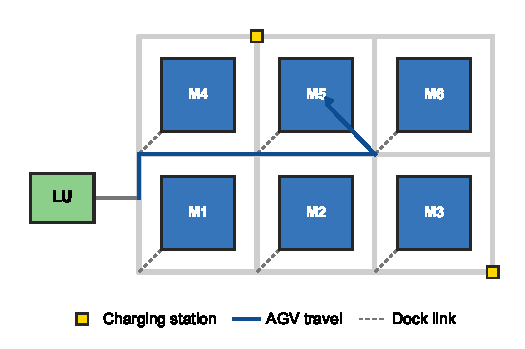
\includegraphics[width=\columnwidth]{fig_layout.pdf}
\caption{Shop layout. Machines occupy grid cells; the aisles are the grid lines
between cells, so a passage never crosses a machine. Each machine has a dock
linking it to the nearest intersection. The load--unload station lies outside
the grid and is joined to the left boundary by one connecting segment. Charging
stations occupy aisle intersections. The solid line is one AGV travel.}
\label{fig:layout}
\end{figure}

Two transport-time calibers coexist in this study, and the caliber is a
property of the instance rather than of the run configuration. Under the
geometric caliber, the travel time between two nodes is the shortest-path
length in the aisle graph divided by the effective vehicle speed. Under the
matrix caliber, the travel time is read from a machine-to-machine travel-time
matrix supplied with the instance; entries are already in minutes, and the
matrix includes the LU station as its zeroth row and column. The matrix is
asymmetric, so a lookup preserves direction. A fleet-wide speed multiplier
still applies under the matrix caliber; the aisle width and the nominal
vehicle speed do not.

\paragraph{Constraints}
Ten constraints are modelled. Each is an independent switch, so a run can
enable any subset.

\begin{description}\itemsep2pt
\item \textbf{C1 --- AGV congestion, zone conflict, deadlock.}
      An aisle segment carries at most one vehicle. A vehicle requests the next
      segment before releasing the previous one, and wait cycles are detected
      and broken.
\item \textbf{C2 --- Finite input and output buffers.}
      A machine blocks when its output buffer is full, and an operation waits
      when the input buffer of its machine is full.
\item \textbf{C3 --- Machine failure.}
      Failures occur at a rate that rises with machine age, and repair occupies
      the machine for a random interval.
\item \textbf{C4 --- Rework.}
      A completed operation is re-queued with probability $p_{\mathrm{rw}}$.
\item \textbf{C5 --- Sequence-dependent setup.}
      A setup time $s_{jj'}$ precedes each job change on a machine.
\item \textbf{C6 --- Due dates and tardiness.}
      Per-job due dates enter Equation~\eqref{eq:twt}. This is the one
      constraint that changes only what is measured: the simulation trajectory
      is unaffected.
\item \textbf{C7 --- AGV failure.}
      A vehicle stops for a repair interval, and tasks already assigned to it
      are returned to the dispatcher and re-offered to the remaining vehicles.
\item \textbf{C8 --- Heterogeneous fleet.}
      Vehicles differ in speed multiplier, load capacity, and battery size.
\item \textbf{C9 --- Charging and battery.}
      Vehicle energy is tracked. A depleted vehicle becomes unavailable, and
      charging is a scheduled decision.
\item \textbf{C10 --- Preventive maintenance.}
      Each machine carries a maintenance clock, and maintenance is a scheduled
      decision that resets it.
\end{description}

The distinction between a constraint that changes the dynamics and one that
changes only the objectives matters for the ablations in
Section~\ref{sec:results}. Switching off a dynamics constraint changes the
trajectory; switching off C6 leaves every trajectory bit-identical and only
removes a term from the objective.

\subsection{Objectives}
\label{sec:problem:objectives}

Three objectives are reported. Let $C_j$ denote the completion time of job
$j$, measured when the job reaches the LU station, and let $d_j$ denote its
due date.

\paragraph{Makespan}
\begin{equation}
\Cmax = \max_{j \in \mathcal{J}} C_j .
\label{eq:makespan}
\end{equation}

\paragraph{Total energy consumption}
Energy is accounted by a three-state machine model and a three-state vehicle
model, plus a fixed shop load. Let $\pi^{\mathrm{p}}_i$, $\pi^{\mathrm{s}}_i$,
and $\pi^{\mathrm{u}}_i$ be the processing, setup, and standby power of machine
$i$, in kilowatts, and let $T^{\mathrm{p}}_i$, $T^{\mathrm{s}}_i$, and
$T^{\mathrm{u}}_i$ be the total minutes machine $i$ spends in each state. Let
$\pi^{\mathrm{l}}$, $\pi^{\mathrm{e}}$, and $\pi^{\mathrm{i}}$ be the loaded,
empty-travel, and standby power of a vehicle, and let $T^{\mathrm{l}}$,
$T^{\mathrm{e}}$, and $T^{\mathrm{i}}$ be the corresponding fleet totals. Let
$P_0$ be the fixed shop power. Then
\begin{equation}
E_{\mathrm{mach}} = \frac{1}{60} \sum_{i \in \mathcal{M}}
   \left( \pi^{\mathrm{p}}_i T^{\mathrm{p}}_i
        + \pi^{\mathrm{s}}_i T^{\mathrm{s}}_i
        + \pi^{\mathrm{u}}_i T^{\mathrm{u}}_i \right),
\label{eq:energy:mach}
\end{equation}
\begin{equation}
E_{\mathrm{agv}} = \frac{1}{60} \left( \pi^{\mathrm{l}} T^{\mathrm{l}}
   + \pi^{\mathrm{e}} T^{\mathrm{e}} + \pi^{\mathrm{i}} T^{\mathrm{i}} \right),
\label{eq:energy:agv}
\end{equation}
\begin{equation}
E_{\mathrm{tot}} = E_{\mathrm{mach}} + E_{\mathrm{agv}}
   + \frac{P_0 \, \Cmax}{60} .
\label{eq:energy}
\end{equation}
The fixed shop load is charged over the makespan, so the third term is linear
in $\Cmax$ by construction.

Section~\ref{sec:results} also reports a second energy account,
$E_{\mathrm{net}}$, which keeps only the terms attributable to the work
actually performed:
\begin{equation}
E_{\mathrm{net}} = \frac{1}{60} \sum_{i \in \mathcal{M}}
   \left( \pi^{\mathrm{p}}_i T^{\mathrm{p}}_i
        + \pi^{\mathrm{s}}_i T^{\mathrm{s}}_i \right)
   + \frac{1}{60} \left( \pi^{\mathrm{l}} T^{\mathrm{l}}
        + \pi^{\mathrm{e}} T^{\mathrm{e}} \right) .
\label{eq:energy:net}
\end{equation}
$E_{\mathrm{net}}$ excludes machine standby, vehicle standby, and the fixed
shop load. The two accounts behave differently as objectives, and
Section~\ref{sec:results} reports that difference as a result rather than
treating the choice as a formality.

\paragraph{Total weighted tardiness}
\begin{equation}
\TWT = \sum_{j \in \mathcal{J}} \wj \max(0, \, C_j - d_j).
\label{eq:twt}
\end{equation}
All job weights are set to one in this study, so \TWT\ is the unweighted total
tardiness. The weights are retained in the formulation because the objective
is defined with them and because the instance data carry a weight field.

\subsection{Due dates}
\label{sec:problem:due}

Due dates must be exogenous, per job, and spread. A common due date makes the
tardiness objective degenerate: if all $d_j$ are equal, then $\TWT = 0$
whenever $\Cmax \le d$, so the objective carries no signal beyond the
makespan. Two formulations that are natural at first sight fail on this point,
and the failure is structural rather than numerical. Setting $d_j$ to a fixed
multiple of the job's own processing time ignores queueing and transport, so
every job is tardy. Setting $d_j = \tau M_{\mathrm{ref}}$, where
$M_{\mathrm{ref}}$ is the makespan of a reference schedule on the same
instance, is endogenous: changing the fleet size changes
$M_{\mathrm{ref}}$ and therefore changes the due dates.

We therefore generate due dates from the job work content. Let
$W_j = \sum_{k} \min_{i \in \mathcal{M}_{j,k}} p_{jki}$ be the shortest
attainable processing time of job $j$, and let
\begin{equation}
\mathrm{LB} = \max \left( \frac{1}{m} \sum_{j \in \mathcal{J}} W_j, \;
   \max_{j \in \mathcal{J}} W_j \right)
\label{eq:lb}
\end{equation}
be a load lower bound on the makespan of any feasible schedule. Let
$\rho_j \in [0,1]$ be the rank of $W_j$ among all work contents, normalized
to the unit interval, with $\rho_j = 0.5$ when $n = 1$. The due date of job
$j$ is
\begin{equation}
d_j = \mathrm{LB} \cdot \tau \cdot \left( 1 + R (2\rho_j - 1) \right).
\label{eq:duedate}
\end{equation}
Equation~\eqref{eq:duedate} reads only instance data: the reference schedule
and the fleet configuration do not appear, so changing the fleet size does not
move any due date. The pair $(\tau, R)$ is calibrated per instance. The
tardiness rate of the reference schedule and the tardiness rate after a 12\%
improvement are both required to fall in $[0.20, 0.75]$; among the pairs that
satisfy this, the calibration selects the one minimizing
$|\eta_{\mathrm{ref}} - 0.45| + |\eta_{\mathrm{imp}} - 0.40| + 0.02R$, where
$\eta$ denotes a tardiness rate. Tightening $\tau$ only increases our own
tardiness, so the rule carries no incentive to tune the target in our favour.
$R$ is bounded below by $0.2$ because $R = 0$ collapses
Equation~\eqref{eq:duedate} to a common due date, which is the degeneracy this
section exists to avoid. It is bounded above by $0.8$ because the factor
$1 + R(2\rho_j - 1)$ crosses zero once $R > 1$, which would produce negative
due dates.

The calibrated $\tau$ differs across instances by up to a factor of 3.4 under
the geometric caliber and 12.0 under the matrix caliber. That spread is
inherent to work-content-based due dates and is reported rather than hidden. Table~\ref{tab:duedates} gives the frozen pairs for both
transport calibers. They are part of the instance data in the sense that
matters here --- the reward of Equation~\eqref{eq:reward} is not reproducible
without them --- so they are reported in full even though the policy results in
this paper come from a single instance.

Both columns were produced by a search over a fixed grid, with a step of 0.05
in $\tau$ and 0.10 in $R$, rather than chosen by hand. Halving the grid step
leaves the induced tardiness rates unchanged on nine of the ten instances under
the geometric caliber; on the tenth it moves to a neighbouring pair with a
slightly worse score. The table reports the frozen values.

\begin{table}[htbp]
\centering
\caption{Frozen due-date parameters, one pair per caliber. The two calibers
measure travel time on different scales, so they need separate pairs.}
\label{tab:duedates}
\setlength{\tabcolsep}{4pt}
\begin{threeparttable}
\begin{tabular}{@{}lrrrr@{}}
\toprule
 & \multicolumn{2}{c}{Geometric} & \multicolumn{2}{c}{Matrix} \\
\cmidrule(r){2-3}\cmidrule(l){4-5}
Instance & $\tau$ & $R$ & $\tau$ & $R$ \\
\midrule
mk01 & 2.75 & 0.3 & 19.80 & 0.4 \\
mk02 & 2.45 & 0.4 & 22.15 & 0.2 \\
mk03 & 3.65 & 0.4 & 16.10 & 0.3 \\
mk04 & 5.00 & 0.7 & 20.45 & 0.5 \\
mk05 & 1.70 & 0.5 &  4.40 & 0.4 \\
mk06 & 5.85 & 0.6 & 45.50 & 0.5 \\
mk07 & 1.90 & 0.5 &  8.60 & 0.3 \\
mk08 & 2.70 & 0.8 &  8.80 & 0.6 \\
mk09 & 2.70 & 0.8 & 13.00 & 0.4 \\
mk10 & 3.10 & 0.8 & 52.70 & 0.6 \\
\bottomrule
\end{tabular}
\begin{tablenotes}\footnotesize
\item Frozen values; the grid search that produced them is described in the
      text.
\end{tablenotes}
\end{threeparttable}
\end{table}

The tardiness objective also saturates. Because due dates are absolute
thresholds, a schedule that finishes every job before the earliest $d_j$
attains $\TWT = 0$ regardless of how much better it is. The calibration above
pins the reference schedule near the middle of the band rather than at either
edge, but the saturation remains, and it is reported wherever it occurs rather
than being treated as a measurement of zero tardiness.

\section{Method}
\label{sec:method}

\begin{figure*}[htbp]
\centering
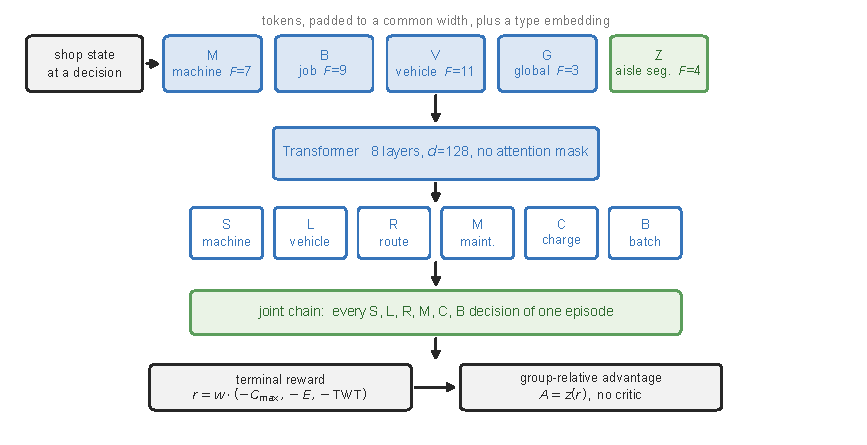
\includegraphics[width=\textwidth]{fig_overview.pdf}
\caption{The policy and its training loop. The shop state at one decision is
encoded as a set of tokens in five segments --- machines, jobs, vehicles, one
global token, and the aisle segments --- padded to a common width and passed
through a Transformer with no attention mask. One head scores the candidates of
each decision kind. Every decision of one episode is appended to a single
chain, which receives one terminal scalarized reward; the group-relative
advantage is computed over the chains sampled at that step, and the policy is
updated without a critic. The zone segment exists only when the congestion
mechanism is enabled; the other four are always present. The zone segment
together with the distance bias and the route head form the
transport-network-aware encoding of Section~\ref{sec:method:state}: they are
what puts the aisle network into the state rather than leaving it to be
inferred from the machine and vehicle tokens.}
\label{fig:overview}
\end{figure*}

\subsection{Overall framework}
\label{sec:method:framework}

Figure~\ref{fig:overview} shows the pipeline, and this subsection names its
stages in the order the running system passes through them.

\emph{Encoding.} At a decision instant the simulation hands over a snapshot:
machine states and buffers, job progress and due-date margins, vehicle
positions and loads, the shop clock, and the aisle occupancy. The snapshot is
turned into the token tensor of Section~\ref{sec:method:state}, with the
per-token features normalized by instance constants so that the same encoder
accepts a 10-job and a 20-job instance.

\emph{Scoring.} The encoder produces one embedding per token. The head of the
active decision kind scores its candidate set against those embeddings, and the
policy samples a candidate during training or takes the highest-scoring one
during evaluation.

\emph{Advancing.} The chosen candidate is applied to the simulation, which runs
until the next decision instant and then hands over a new snapshot. The chain
grows by one decision. The kind of the next decision is determined by the
triggering event, not by a fixed schedule, so the proportion of S, L, and
optional decisions in a chain is a property of the episode rather than a design
constant.

\emph{Learning.} The episode ends, one terminal reward is computed, and the
chains sampled at that step are compared with one another to give the advantage
of Algorithm~\ref{alg:train}.

\emph{Deployment.} At inference the policy needs the same snapshot, the same
candidate construction, and one forward pass; it does not need the reference
run, the reward, or the group. The candidate sets are built from the simulation
state exactly as during training, so the action space seen at deployment
matches the one seen during training. Evaluation in this paper uses argmax
action selection, which makes a trained policy deterministic given a seed; the
group-based sampling path exists only during training.

\subsection{Markov decision process formulation}
\label{sec:method:mdp}

We formulate the coupled problem as a Markov decision process
$\mathcal{M} = (\mathcal{S}, \mathcal{A}, P, r, \gamma)$ with a terminal
reward and no discounting.

\paragraph{State}
At a decision instant $t$ the state is the shop snapshot, encoded as a token
tensor and a segment assignment,
\begin{equation}
s_t = \left( \mathbf{X}_t \in \mathbb{R}^{N \times F_{\max}}, \;
            \mathbf{g}_t \in \{1,\dots,5\}^{N} \right),
\label{eq:state}
\end{equation}
where $N = m + n + V + 1 + Z$ is the number of tokens, $F_{\max}$ the padded
feature width, and $\mathbf{g}_t$ the segment identifier of each token. The
token set is built from the simulation state at the instant of the decision,
not from a fixed initial snapshot, so a decision taken late in an episode sees
the consequences of the decisions taken before it.
Section~\ref{sec:method:state} lists the features.

\paragraph{Action}
The action space is not a single set, because the decisions are of different
kinds. At each decision instant exactly one kind $k$ is active, drawn from
$\mathcal{K} = \{\mathrm{S}, \mathrm{L}, \mathrm{R}, \mathrm{M}, \mathrm{C},
\mathrm{B}\}$, and the action is a choice from a candidate set that depends on
the state and the kind:
\begin{equation}
a_t \in \mathcal{C}_k(s_t), \qquad
\mathcal{C}_k(s_t) = \{c_1, \dots, c_{C}\}, \quad C = C_k(s_t).
\label{eq:action}
\end{equation}
The candidate set varies in size: eligible machines for an operation, available
vehicles for a transport task, admissible paths for a travel, admissible batch
sizes for a pick-up. Formulating the action this way, rather than as a fixed
index into a problem-sized vector, is what lets one parameter set serve
instances of different size.

\paragraph{Transition}
$P(s_{t+1} \mid s_t, a_t)$ is the discrete-event simulation itself. The shop
advances until the next decision instant, and the triggering event --- an
operation released, a travel requested, a machine idle, a vehicle empty, a
batch starting --- determines the kind $k$ of the next decision. Because the
simulation is stochastic (failures, rework, repair durations), the transition
is stochastic even when the policy is deterministic.

\paragraph{Reward}
The reward is terminal and arrives once, at the end of the episode:
\begin{equation}
r(s_1, a_1, \dots, a_T) = w_1(-\Cmax) + w_2(-E) + w_3(-\TWT),
\label{eq:reward-mdp}
\end{equation}
with the weights of Equation~\eqref{eq:weights}. There is no intermediate
reward and no shaping term, so the credit for every decision in an episode is
assigned by the same scalar.

\paragraph{Objective}
The policy $\pi_\theta(a_t \mid s_t)$ is trained to maximize
$\mathbb{E}_{\pi_\theta}[r]$, with no discount factor, since the horizon is
the episode.

\subsection{Joint-chain formulation}
\label{sec:method:chain}

An episode of the scheduling problem contains many decisions of more than one
kind. Each operation needs a machine, and each transport task needs a vehicle.
A policy could be trained on each decision point separately, with one reward
per decision. We instead treat the whole episode as one decision chain.

Let $a_S$ be the sequence of machine choices, one per operation, and $a_L$ the
sequence of vehicle choices, one per transport task. A \emph{chain} is the pair
$(a_S, a_L)$ together with the optional decisions of
Section~\ref{sec:method:mechanisms}. Its log-probability under the policy is the
sum of the per-decision log-probabilities,
\begin{equation}
\begin{split}
\logp(\text{chain})
   &= \sum_{t} \logp_S(a_S[t] \mid s_t)
      + \sum_{t} \logp_L(a_L[t] \mid s_t) \\
   &\quad + \sum_{k} \sum_{t} \logp_k(a_k[t] \mid s_t),
\end{split}
\label{eq:chain-logp}
\end{equation}
where the last sum runs over the optional decision kinds $k$ that are enabled.
The chain receives a single terminal reward, computed after the episode ends.
No intermediate reward is used.

Three properties of the problem motivate this formulation.

First, group-relative advantages compare the members of a group with one
another. That comparison is only meaningful if every member was produced by the
same policy from the same state distribution. If the production and logistics
decisions were split between two policies, each group would mix samples drawn
from two different distributions, and the group mean would no longer estimate
a baseline for either of them. Multi-agent methods handle this by learning a
joint value function or a centralised critic~\citep{rashid2018qmix,yu2022mappo};
both routes reintroduce the critic that a group-relative method is meant to
avoid.

Second, the two decision layers are coupled by construction: the quality of a
dispatching decision depends on the production plan that generated the
transport tasks. A dispatching policy that is trained against a fixed or
randomly generated plan therefore learns against a task stream that the
deployed system will not produce.

Third, the coupling is asymmetric. Production decisions determine which
transport tasks exist and when they exist; transport decisions determine
whether the machines receive work on time. A chain-level advantage assigns
credit to the whole chain and leaves the split between the two layers to the
policy.

Treating a trajectory as one object and learning from it as a sequence is
itself an established formulation~\citep{chen2021decision}. What is specific
here is that the sequence spans two decision layers whose actions are of
different kinds and live in different candidate spaces, and that the reward
arrives only at the end. The candidate-scoring interface of
Section~\ref{sec:method:policy} is what lets one chain carry both.

\subsection{State representation}
\label{sec:method:state}

The policy reads the shop state as a sequence of tokens. Four kinds of entity
are encoded, plus one global token. Each token carries a fixed-width feature
vector. The feature vectors of the four segments are padded to a common width
$F_{\max}$ and concatenated into a single tensor of shape $(N, F_{\max})$, where
$N = m + n + V + 1$ for $m$ machines, $n$ jobs, and $V$ vehicles. A segment
identifier accompanies the tensor.

Machines, jobs, vehicles, and the global token have different numbers of
informative fields. A machine has 7, a job has 9, a vehicle has 11, and the
global token has 3. Because the four segments are padded to a common width,
column $c$ of a machine token and column $c$ of a job token can carry different
meanings. A learned type embedding, indexed by the segment identifier, is added
to every token and is what separates those meanings. Without it the shared
projection cannot distinguish a machine from a job.

Table~\ref{tab:features} lists the features. All quantities are normalized by
static instance constants --- total work content, the makespan of a reference
schedule, the machine count, the bounding box of the shop --- rather than by
per-episode statistics, because online decision making cannot observe the
statistics of an episode that has not finished.

\paragraph{Transport-network-aware encoding}
The four segments above describe the machines, the jobs, and the vehicles, and
none of them carries the shop's spatial structure: a machine token says how
much work is queued, not how far it is from anything else. We therefore add the
transport network to the state, in three parts that only work together. The
aisle segments become a fifth token segment, so each segment of the network is
an entity carrying its own occupancy and the time vehicles have waited on it. A
distance-dependent bias enters the attention score, so that a token can be
attended to in proportion to how far its entity is from the deciding one. And
the route head reads the segment tokens its candidate path would traverse,
which is what turns the first two parts from context into something the policy
can choose between. Section~\ref{sec:method:mechanisms} lists the switches that
enable each part.

This is a representation choice and not a claim about generalization. Whether
the encoding transfers to a shop layout it was not trained on is a separate
question, and this paper does not measure it.

\begin{table*}[htbp]
\centering
\caption{Token features. Each column is one scalar. Normalizers are instance
constants, not per-episode statistics.}
\label{tab:features}
\setlength{\tabcolsep}{4pt}
\begin{threeparttable}
\begin{tabular}{@{}llp{11.4cm}@{}}
\toprule
Segment & Width & Features \\
\midrule
Machine ($m$ tokens) & 7 &
  Queued processing work divided by total work content;
  queued operations divided by input capacity;
  output buffer occupancy divided by output capacity;
  busy indicator and remaining processing time as a fraction of the operation;
  remaining time until the next forced maintenance;
  failure rate divided by the largest failure rate in the instance. \\
Job ($n$ tokens) & 9 &
  Completed operations divided by total operations;
  remaining nominal processing time divided by total work content;
  due-date margin $(d_j - \text{now})/M_{\mathrm{ref}}$, which may be negative;
  completion indicator;
  current machine index, normalized, or $-1$ if not started;
  in-transit indicator and the index of the carrying vehicle;
  job weight divided by the largest weight. \\
Vehicle ($V$ tokens) & 11 &
  One-hot over idle, empty-travelling, loaded, and failed;
  current node coordinates divided by the bounding-box diagonal;
  assigned tasks divided by the instance maximum;
  battery fraction;
  load divided by capacity;
  speed multiplier divided by the largest multiplier;
  time spent waiting for an aisle segment divided by the wait limit. \\
Global (1 token) & 3 &
  Elapsed time divided by $M_{\mathrm{ref}}$;
  completed jobs divided by $n$;
  tasks in transit divided by the instance maximum. \\
\bottomrule
\end{tabular}
\begin{tablenotes}\footnotesize
\item The setup time of a job change is deliberately absent from the machine
      token. Setup is a property of a machine--job pair, not of either entity
      alone, so it is supplied to the machine-selection head as a candidate
      feature instead. A per-entity feature cannot express it.
\end{tablenotes}
\end{threeparttable}
\end{table*}

\subsection{Policy architecture}
\label{sec:method:policy}

The encoder is a standard Transformer~\citep{vaswani2017}. Tokens are
projected, given a type embedding, and passed through $L$ self-attention layers
with no mask, so every token can attend to every other token. We use $L = 8$
layers and model dimension $d = 128$ throughout.

Attention is unmasked rather than restricted to within-segment or
within-axis blocks. Segment identity is information about what a token is;
an attention mask is a restriction on what a token may see. The two are not
interchangeable, and dropping a restriction does not drop the information.

Each decision kind has its own head. A head scores \emph{candidates} rather
than a fixed action set, in the manner of pointer
networks~\citep{vinyals2015pointer}:
\begin{equation}
\ell = f_k\!\left(\mathbf{h}_{\text{token}}, \mathbf{g}_{\text{decision}},
   \mathbf{c}_{1:C}\right) \in \mathbb{R}^{C},
\label{eq:candidate}
\end{equation}
where $\mathbf{h}_{\text{token}}$ is the encoder output for the token that
owns the decision, $\mathbf{g}_{\text{decision}}$ collects decision-level
features, and $\mathbf{c}_{1:C}$ are per-candidate features. The number of
candidates $C$ varies with the state and with the instance, so the same
parameters serve a 10-job and a 20-job instance without resizing. Every head
reads the same token embeddings; no head receives a hand-built flat vector.

This matters because the candidate count is not a design constant. Eligible
machines per operation, available vehicles per task, viable paths per travel,
and admissible batch sizes all vary from decision to decision. Attention over
a set of elements is permutation-invariant by construction~\citep{lee2019set},
which is the property the head relies on: the score of a candidate must not
depend on where in the candidate list it happens to sit.

\subsection{Group-relative training over chains}
\label{sec:method:training}

For each training step the policy samples $G$ chains from the same state. Each
chain $g$ yields a terminal reward $r_g$. The advantage is the group-relative
score of Shao et al.~\citep{shao2024grpo},
\begin{equation}
A_g = \frac{r_g - \operatorname{mean}(r_{1:G})}
           {\operatorname{std}(r_{1:G}) + \epsilon},
\label{eq:advantage}
\end{equation}
and the objective is the REINFORCE objective with this advantage,
\begin{equation}
\mathcal{L} = -\frac{1}{G} \sum_{g=1}^{G} A_g \,
   \logp(\text{chain}_g),
\label{eq:loss}
\end{equation}
with $\logp$ from Equation~\eqref{eq:chain-logp}. No critic is used. The
optimizer is Adam. A single group is used per step ($J = 1$); the sampling
budget is spent on $G$ rather than on repeated seeds, because the group mean
already supplies the baseline and averaging over seeds would reduce noise
inside a quantity that is about to be compared within the group. The group is
also where diversity comes from: all $G$ chains start from the same state and
differ only in the sampling, the same device that multi-start policy
optimization uses to find several good solutions to one
instance~\citep{kwon2020pomo}.

\begin{algorithm}[t]
\caption{Joint-chain group-relative policy optimization}
\label{alg:train}
\begin{algorithmic}[1]
\Require instance, initial policy $\pi_\theta$, group size $G$, steps $T$
\Statex \textbf{reference} run the reference schedule once, cache
       $f^{\mathrm{ref}}$, $w$, $M_{\mathrm{ref}}$
\For{step $= 1$ \textbf{to} $T$}
  \For{$g = 1$ \textbf{to} $G$}
    \State sample a chain $\tau_g$: run the simulation under $\pi_\theta$
    \Statex \hspace{\algorithmicindent} and record every S, L, R, M, C, B decision
    \State $r_g \gets w_1(-\Cmax^{(g)}) + w_2(-E_g) + w_3(-\TWT_g)$
  \EndFor
  \State $\bar{r} \gets \frac{1}{G}\sum_{g} r_g$; \quad
         $\sigma \gets \sqrt{\frac{1}{G}\sum_{g} (r_g - \bar{r})^2}$
  \State $A_g \gets (r_g - \bar{r}) \,/\, (\sigma + \epsilon)$
         \Comment{advantage, Eq.~\eqref{eq:advantage}}
  \State $\mathcal{L} \gets -\frac{1}{G}\sum_{g} A_g \logp(\tau_g)$
  \State $\theta \gets \mathrm{Adam}\!\left(\theta, \nabla_\theta \mathcal{L}\right)$
\EndFor
\end{algorithmic}
\end{algorithm}

\paragraph{Training details}
The reference run is executed once per instance and configuration, and the
weights of Equation~\eqref{eq:weights} are derived from it before training
starts; the same run supplies the normalizing constant $M_{\mathrm{ref}}$ used
in the token features, so features and reward share one reference point.
Training uses $G = 8$ chains per step, $T = 300$ steps, Adam with a learning
rate of $3\times10^{-4}$, and a single pass over each group
($\mathrm{epochs} = 1$, so the default path is REINFORCE with a group-relative
advantage). Action sampling uses a seeded generator derived from the chain
index, which makes a run reproducible within one process but not across
processes. Evaluation uses argmax action selection over five perturbation
seeds, none of which is seen during training.

Equation~\eqref{eq:advantage} divides by the group standard deviation.
Section~\ref{sec:results} reports an ablation over this choice: a variant that
subtracts the group mean without dividing by the standard deviation, and a
variant that uses the raw reward. The three variants differ only in the
advantage; every switch and hyperparameter is otherwise identical. The same
comparison has been made for neural combinatorial optimization, where the
group-relative construction is used without a critic as
well~\citep{sepulveda2026baselinefree}, and the constrained variant of the same
family is what our budget mechanism
extends~\citep{hu2023constrained,achiam2017cpo,tessler2019rcpo}.

\paragraph{Reward}
The reward is a weighted scalarization of the three objectives,
\begin{equation}
r = w_1 (-\Cmax) + w_2 (-E) + w_3 (-\TWT),
\label{eq:reward}
\end{equation}
with weights derived from a reference schedule rather than chosen by hand:
\begin{equation}
w_i = \frac{1/f_i^{\mathrm{ref}}}{\sum_j 1/f_j^{\mathrm{ref}}},
\label{eq:weights}
\end{equation}
where $f_i^{\mathrm{ref}}$ is the measured value of objective $i$ under the
reference schedule. The reference schedule assigns every operation to its
fastest eligible machine and dispatches vehicles round-robin. The weights are
normalized so that improving each objective by one unit relative to the
reference contributes equally. We report the weight vector together with the
reference schedule, because the tardiness component of $f^{\mathrm{ref}}$
depends on the due-date calibration and the reward is not reproducible without
it.

Combining the objectives at the reward level keeps one scalar return per
episode, which is what the advantage estimator operates on; combining them at
the gradient level~\citep{sener2018mgda,yu2020pcgrad} would instead require
per-objective advantages and a rule for reconciling them.

The reward is terminal and undiscounted, and no shaping term is
added~\citep{ng1999shaping}. This is a deliberate simplification: a shaping
term would require a potential function over a state space in which the useful
potential is not obvious, and it would change what the episode-level comparison
inside a group means.

\subsection{Constraint mechanisms}
\label{sec:method:mechanisms}

Ten constraints are modelled. Making them switchable is not enough to make them
learnable; the policy must also be able to act on them. We group the mechanisms
by what they change.

\begin{itemize}
\item \textbf{Decision points.} The mechanism adds a new kind of decision that
      was previously made by a fixed rule, and the policy chooses it. The
      candidate-scoring interface of Equation~\eqref{eq:candidate} is what makes
      this a local change: a new head is added, the chain grows, and nothing
      else moves.
\item \textbf{Dynamics.} The mechanism changes how the shop evolves --- a
      breakdown, a returned task, a blocked buffer. The policy does not gain an
      action; it faces a different system.
\item \textbf{Input.} The mechanism adds features to the representation. No
      action and no trajectory changes.
\end{itemize}

The mechanisms are listed below. Every switch defaults to off,
and turning it off reproduces the pre-mechanism behaviour bit for bit; that
property is verified rather than asserted (Section~\ref{sec:setup:repro}).

\begin{description}\itemsep2pt
\item \textbf{Route choice (C1, decision point, \texttt{route\_k}).}
      At each travel the policy selects one of the $k$ shortest paths between
      the endpoints. Candidates carry path length, the number of aisle segments
      traversed, and the current contention on those segments.
\item \textbf{Zone tokens (C1, input, \texttt{route\_zones}).}
      Aisle segments become tokens, and the route head reads the segments its
      candidate traverses. Without this, the candidates of a travel differ only
      in their own summary features.
\item \textbf{Geometric bias (C1, input, \texttt{geom\_bias}).}
      A fixed, non-learned bias $-w\,d(i,j)/\text{diag}$ is added to the
      attention score, where $d$ is the shortest-path distance on the aisle
      graph. Nothing is learned here; the term only makes distance and
      congestion visible to attention.
\item \textbf{Maintenance head (C10, decision point, \texttt{pm\_head}).}
      When a machine is idle the policy chooses between starting maintenance
      now and deferring it. The forced-maintenance threshold remains a hard
      floor, so the policy can advance maintenance but not postpone it.
\item \textbf{Charging head (C9, decision point, \texttt{charge\_head}).}
      When a vehicle is idle the policy chooses between not charging and each
      charging station. A vehicle whose battery reaches zero becomes
      unavailable until it recovers.
\item \textbf{Multi-drop travel (C8, dynamics, \texttt{multi\_drop}).}
      One trip collects every queued task at a pick-up point and delivers to
      several drop points, bounded by capacity. Loaded travel becomes a
      sequence of segments rather than one.
\item \textbf{Batch head (C8, decision point, \texttt{batch\_head}).}
      At pick-up the policy chooses how many further tasks to append to the
      trip. Candidates carry batch size, the number of tasks whose relative
      order the batch would disturb, and the resulting travel saving.
\item \textbf{Failure failover (C7, dynamics, \texttt{agv\_failover}).}
      Tasks held by a failed vehicle are returned and offered to vehicles that
      are still running.
\item \textbf{Age-dependent failure (C3, dynamics, \texttt{machine\_age\_failure}).}
      The failure rate rises with the machine maintenance clock along a Weibull
      hazard, so the failure process acquires memory and maintenance acquires a
      second effect.
\end{description}

Four constraints need no dedicated mechanism. C2, C4, and C6 are already
visible in the token features of Table~\ref{tab:features}, and C5 is supplied
to the machine head as a candidate feature. Section~\ref{sec:results} reports
which of the mechanisms changed a measured quantity and which did not.

\paragraph{Why some ablation arms change more than one switch.}
A decision point that is enabled while the constraint it acts on is disabled
produces a dead action: the head samples a choice that cannot change anything,
and the chain log-probability still includes it. The advantage would then be
assigned partly to a decision with no effect, which contaminates the comparison
rather than merely wasting computation. Such combinations are therefore
rejected rather than permitted, and the consequence for the ablations is that
several arms necessarily change more than the one item they are named for. The
logistics arm, for instance, also disables the route head, the zone tokens, the
charging head, and the batch head, because each of those acts on a constraint
the arm has switched off. The released configuration files record the exact
switch set of every run, and Table~\ref{tab:ablation} marks the affected arms
so that the reader is not left to infer the switch set from the arm name.

\paragraph{Two mechanisms change the simulated system, not only the policy.}
Making vehicle capacity operational required changing the travel model: one
trip now collects every queued task at a pick-up point and delivers to several
drop points, so loaded travel is a sequence of segments rather than one. This
is a change to the shop dynamics and it is reported as such, because it means
the readings on either side of it are not comparable. The same is true of the
charging mechanism, which required that a vehicle at zero battery actually
become unavailable before there was a decision worth making. Both changes were
made because a parameter the model carried --- load capacity, battery state ---
had no effect on the simulation. The list below marks each
mechanism as a decision point, a dynamics change, or an input change for
exactly this reason.

\subsection{Lagrangian constraint budgets}
\label{sec:method:t3}

A constraint that is modelled but never violated contributes nothing to the
reward, so the policy has no reason to avoid violating it when the trade-off
turns favourable. We add a Lagrangian term with a per-constraint multiplier.
The construction follows the constrained policy optimization
lineage~\citep{achiam2017cpo,tessler2019rcpo}, with one difference that matters
here: those methods estimate the constraint cost with a value function, and we
do not use a critic. The multiplier is updated from the batch itself, which is
what makes the scheme compatible with a group-relative advantage.

Let $a_i$ be the activation of constraint $i$ over an episode, measured so
that it counts only what the policy was forced into: time spent waiting for an
aisle segment, minutes blocked by a full buffer, setup minutes, failures,
battery-depletion events, and maintenance triggered by the threshold. Let
$a_i^{\mathrm{ref}}$ be the same quantity under the reference schedule, so that
$\hat a_i = a_i / a_i^{\mathrm{ref}}$ is the activation as a fraction of the
reference level. With a budget $b_i$, the penalized reward of chain $g$ is
\begin{equation}
r'_g = r_g - \sum_i \lambda_i \hat a_{i,g},
\label{eq:lagrangian}
\end{equation}
and the advantage is computed from $r'$ as in Equation~\eqref{eq:advantage}.
The multipliers follow dual ascent,
\begin{equation}
\lambda_i \leftarrow \operatorname{clip}\!\left(
   \lambda_i + \eta \left(\hat a_i - b_i\right), \, 0, \, \lambda_{\max}\right),
\label{eq:dual}
\end{equation}
where $\hat a_i$ is the mean over the group, $\eta$ is a step size, and
$\lambda_{\max}$ guards against divergence. The multipliers persist across
training steps; they are not reset per step.

Two properties of this construction need to be stated because they bound what
it can do. The penalty is applied to the scalar reward \emph{before} the group
normalization, so the effective strength of $\lambda_i$ is scaled by the group
standard deviation of the reward and is not a direct statement of how much
weight the constraint carries. And the penalty enters the advantage only if the
group can express a difference: with $G = 2$ the normalized advantage is
identically $(-1,+1)$ regardless of the reward, so the penalty is inert. The
budget mechanism therefore requires $G \ge 3$.

Two constraints are excluded from the budget. Rework and vehicle failure are
memoryless events that the policy cannot influence, so penalizing them would
add noise to the reward rather than pressure to the policy. For the same
reason a constraint is admitted only when the policy has the corresponding
action available; the configuration is rejected at start-up if a constraint in
the budget has no enabled mechanism to act on it.

\paragraph{Calibration and the meaning of the budget.}
The reference activation $a_i^{\mathrm{ref}}$ is measured on the reference
schedule, and the budget $b_i$ is expressed as a fraction of it. The scale of
$a_i$ differs by three orders of magnitude across constraints --- aisle waiting
is measured in minutes, maintenance in events --- which is why the ratio form
is used rather than the raw quantity.

Calibration is done in a configuration in which all six constraints activate,
because on the standard parameters two of them never do
(Section~\ref{sec:results:active}) and a ratio with a zero denominator is
undefined. On the geometric caliber all ten instances yield six live
constraints. On the matrix caliber only four of the ten instances do, because
in the remaining six the buffer-blocking quantity is identically zero on the
reference schedule; those instances are excluded from the table rather than
entering it with an undefined reference, and a lookup on an absent instance
raises an error instead of falling back.

\paragraph{What the budget can and cannot reach.}
The penalty is computed from the activation of constraints in the
configuration being trained, not from the calibration configuration. If a
constraint never activates in training, its normalized activation is zero while
its reference is not, so its multiplier stays at zero and the constraint is not
penalized. Under the standard parameters this happens for two of the six
constraints, so the budget in practice acts on four of them. This is stated in
Section~\ref{sec:results:active} and is reflected in the way the budget arm is
described there.

\subsection{Computational cost}
\label{sec:method:cost}

The policy is evaluated once per decision, and a decision costs one forward
pass over the token sequence plus the construction of its candidate set. The
network dominates the cost of a step: across the configurations we measured,
the sampling pass, the recomputation pass, and the backward pass together
account for between 55 and 88 per cent of a step, and the simulation for the
remainder. Costs are reported per training step, each step comprising $G = 8$
sampled episodes and one update.

With the mechanisms switched off, a step costs between 0.85\,s and 6.00\,s
depending on instance size, and a step over all ten instances of the benchmark
costs 26.4\,s in total. The cost grows with the number of decisions per episode
rather than with the number of tokens, since each S and L decision is a
separate forward pass; the 20-job instances cost roughly five times the 10-job
instance for that reason.

The optional mechanisms add measured overhead, and one of them reduces cost.
Enabling the aisle-segment tokens multiplies the cost of a step by about 1.44,
because they lengthen the token sequence and the route head reads a subset of
them per candidate. The distance bias adds about 5\%, since the bias is
precomputed. Multi-drop travel and the batch head together add about 2\% on
MK01 and 7\% on MK10. Chunking the log-probability recomputation, by contrast,
reduced both memory and time on the largest instance: without it the peak
allocation reached 49.6\,GB and the run could not complete on the available
device, and with a chunk size of 128 the peak fell to 1.3\,GB and the step
became 1.36 times faster. All figures are single measurements on one machine
and are reported with their configurations in the released records; they should
be read as orders of magnitude rather than as benchmarks.

\section{Experiments}
\label{sec:experiments}

\subsection{Experimental settings}
\label{sec:setup}
\subsubsection{Benchmark instances}
\label{sec:setup:instances}

Instances come from the MKT benchmark~\citep{homayouni2021}, which takes the
processing data of the Brandimarte MK instances~\citep{brandimarte1993}
unchanged and adds two things: a machine-to-machine travel-time matrix and a
vehicle count. The matrices are asymmetric, and their zeroth row and column
address the load--unload station. Adding transport to the MK data does not
alter any processing time, so results can be traced back to the original
instances.

This paper reports results on MK01 only: 10 jobs, 6 machines, 55 operations.
We state this plainly because it bounds every claim below. The remaining
instances of the benchmark are not covered here, and no statement in this paper
should be read as extending to them.

One property of MK01 matters for the interpretation of the results. Of the
instances in the benchmark, MK01 offers the fewest opportunities for
multi-drop travel: the instance can batch more than one task on 1.4\% of its
pick-ups, against 2.5\% for MK07 and 12.3\% for MK10. A mechanism that only
acts when a batch can be formed will therefore look inert on MK01 for reasons
that belong to the instance rather than to the mechanism. We report the
batching results with that caveat attached rather than as a verdict on the
mechanism.

\subsubsection{Configuration}
\label{sec:setup:config}

Two report tiers are used throughout. Tier A (\texttt{A-MKT}) switches off all
ten constraints and all mechanisms, leaving a flexible job shop with transport.
Tier B (\texttt{B-Full}) enables all of them. The two tiers differ only in the
mechanism switches; the instance, the fleet size, and the transport caliber are
identical.

All policies are trained for 300 steps with a group size of $G = 8$, learning
rate $3\times10^{-4}$, and Adam, on a single training seed ($\text{seed} = 0$).
The policy is evaluated every 30 steps on five evaluation seeds with argmax
action selection. The training seed is the only source of variation in the
learned parameters; the five evaluation seeds perturb the simulation, not the
training.

We report the training-seed variation explicitly, because it is large. Under
the \texttt{scalar} advantage with the budget mechanism off, five training
seeds on MK01 give makespans of 84.04, 81.24, 87.19, 79.27, and 71.56 --- a
mean of 80.66, a standard deviation of 5.90, and a range of 15.63. Every
ablation number in Section~\ref{sec:results} other than the advantage ablation
comes from a single training seed, and the differences between ablation arms
are of the same order as that standard deviation. Those numbers are reported as
measurements, not as effect estimates, and are labelled as single-training-seed
throughout. The advantage ablation (Section~\ref{sec:results:advantage}) is the
exception: all three of its arms were trained with five seeds, precisely because
its conclusions are not readable from one.

\subsubsection{Baselines}
\label{sec:setup:baselines}

Three baselines are used.

\begin{itemize}
\item \textbf{Rule.} Each operation goes to its fastest eligible machine, with
      a first-in-first-out tie-break, and vehicles are dispatched round-robin.
      This is also the schedule used to derive the reward weights of
      Equation~\eqref{eq:weights}, so it defines the reference point that the
      reward is normalized against.
\item \textbf{Single-objective GRPO.} The same policy and training procedure,
      with the preference vector set to a one-hot vector over one of the three
      objectives. Three arms are trained, one per objective. This is the
      standard scalarization control: it answers whether training on the
      weighted scalar is better or worse than training once per objective and
      choosing afterwards.
\item \textbf{NSGA-II.} Population 100, 50 generations, 5000 evaluations per
      tier, run on the same instance and the same fleet and constraint
      configuration as the learned policies.
\end{itemize}

A fourth baseline layer --- a published deep reinforcement learning method ---
is not included. The comparison is therefore restricted to a rule, a
single-objective version of our own method, and a metaheuristic.
Section~\ref{sec:discussion} records what this omission costs.

\paragraph{Out-of-sample re-evaluation of the front}
NSGA-II searches on a single random chain. Points found on that chain can
overfit it. Every point of the NSGA-II front is therefore re-evaluated on the
same five evaluation seeds used for the policies, and the re-evaluated front is
what we compare against. The difference is not cosmetic: on tier B the search
front reads $78.09$ in-sample and $79.56$ after re-evaluation, and individual
front points move further ($78.18 \rightarrow 88.62$).

\paragraph{Matching the baselines to the tier}
The rule baseline is run under the same constraint set as the policy it is
compared with, using the same five evaluation seeds, so that comparisons
between the rule row and the policy row are paired. The rule makespan under
tier B (105.35) and under tier A (73.01) are therefore different quantities,
and neither equals the reference makespan used for the reward weights.

\subsubsection{Reproducibility}
\label{sec:setup:repro}

Every mechanism switch defaults to off, and a run with all switches off
reproduces the pre-mechanism trajectory bit for bit. This property is what
makes the ablations in Section~\ref{sec:results} measurements of the mechanism
rather than of an incidental change elsewhere, so it is verified rather than
asserted: a digest of the sampled chain and of the parameter vector is pinned
for each switch position, and the same discipline is applied to the wiring
between training and evaluation, so that a switch cannot be active in one and
inactive in the other.

Because the switches alter the shop dynamics, the reference makespan differs
between ablation arms. Disabling age-dependent failure changes the reference
makespan from 109.05 to 117.77; disabling multi-drop travel changes it to
115.13. The absolute makespan of an arm that switches off a dynamics constraint
is therefore not comparable with the absolute makespan of an arm that leaves it
on: the two arms solve different problems. Where such a comparison would be
misleading we report the paired difference against the all-on configuration
instead.

\subsubsection{Why published figures are not reproduced in our tables}
\label{sec:related:incomparable}

We deliberately do not place our numbers in a table beside published numbers
from this literature. Four differences independently prevent the comparison,
and each one is large enough to change the conclusion on its own.

\emph{Travel-time caliber.} Some published results use a machine-to-machine
travel-time matrix and others use geometric travel times. We use both, and the
caliber is a property of the instance rather than a run-time switch, so a
number cannot be moved between calibers by changing a configuration. The same
chromosome evaluated under a geometric caliber and under a matrix caliber
differs by roughly a factor of four in our own measurements.

\emph{Fleet size.} Our main configuration uses three vehicles. Published
results on the same instance family use six or use the number of machines. The
vehicle count is not published with the benchmark: the source
paper~\citep{homayouni2021} describes it as a uniform draw over a range of the
machine count, so any specific value used by a later paper is a reconstruction
rather than a reproduction.

\emph{Simulator.} Each study runs its own discrete-event simulation. Two
simulators that agree on the problem statement can disagree on makespan through
tie-breaking, event ordering, and rounding.

\emph{Transport boundary.} Our makespan includes the travel of a job from the
load--unload station to its first machine and its return travel after its last
operation. Published makespans in this line end at the completion of the last
operation. The difference is measurable and not small.

Because these four differences are independent, no single adjustment corrects
for them all, and a table that placed the numbers side by side would invite a
comparison that the numbers cannot support. We therefore compare only against
baselines we ran ourselves on our own configuration, and we state the boundary
explicitly rather than leaving it to a footnote. The consequence for evaluation
is that this paper cannot claim to have beaten a published method; it can claim
to have measured its own method against a rule, a single-objective version of
itself, and a metaheuristic, all under one caliber.
Section~\ref{sec:discussion} records what that costs.

\label{sec:results}

\subsection{Main comparison}
\label{sec:results:main}

Table~\ref{tab:main} reports the three baselines against the learned policy on
both tiers. The $\pm$ values are the spread over the five evaluation seeds.

\begin{table*}[htbp]
\centering
\caption{Main comparison on MK01. Tier A disables all ten constraints and all
mechanisms; tier B enables them. The
rule row is run under the same constraint set as the policy it is paired with,
so the two rule rows are not the same quantity. NSGA-II rows are re-evaluated
out-of-sample on the five evaluation seeds.}
\label{tab:main}
\setlength{\tabcolsep}{5pt}
\begin{threeparttable}
\begin{tabular}{@{}llrrrr@{}}
\toprule
Tier & Method & Makespan & Energy (\kWh) & \TWT & Source \\
\midrule
A & Rule (same constraint set) & 73.01 $\pm$ 0.00 & 5.675 & 0.000 & --- \\
A & Single-objective GRPO, makespan & 57.60 & 4.714 & 0.000 & --- \\
A & Single-objective GRPO, energy & 52.91 & 4.341 & 0.000 & --- \\
A & \textbf{Ours} (weighted scalar) & 49.27 & 4.097 & 0.000 & --- \\
A & NSGA-II (out-of-sample) & \textbf{49.14} & \textbf{4.093} & 0.000 & --- \\
\midrule
B & Rule (same constraint set) & 105.35 $\pm$ 4.56 & 7.936 $\pm$ 0.33 & 60.14 $\pm$ 19.00 & --- \\
B & Single-objective GRPO, makespan & \textbf{74.09} $\pm$ 4.67 & 5.790 & 5.977 & --- \\
B & Single-objective GRPO, energy & 96.93 $\pm$ 9.98 & 7.434 & 97.458 & --- \\
B & Single-objective GRPO, \TWT & 77.30 $\pm$ 6.35 & 6.048 & 7.392 & --- \\
B & \textbf{Ours} (weighted scalar) & 78.90 $\pm$ 3.71 & \textbf{6.160} & \textbf{5.042} & --- \\
B & NSGA-II (out-of-sample) & 79.56 $\pm$ 2.64 & 6.239 & 42.48 & --- \\
\bottomrule
\end{tabular}
\begin{tablenotes}\footnotesize
\item Tier A switches off the tardiness constraint, so \TWT\ is identically
      zero for every row of tier A by definition, not as a measurement. Tier A
      also has no stochastic source left once the ten constraints are off, so
      its five evaluation seeds return identical values and no statistical test
      is possible on that tier. The tier A NSGA-II row is deterministic and
      rests on 5000 evaluations.
\end{tablenotes}
\end{threeparttable}
\end{table*}



On tier B the learned policy dominates the entire NSGA-II front: the front's
best re-evaluated values are 79.56 for makespan, 6.239 for energy, and 20.73
for tardiness, and the policy attains 78.90, 6.160, and 5.042. Every one of the
12 re-evaluated front points is dominated. The rule baseline is beaten by
26.5 in makespan and by 55.1 in tardiness.

On tier A the ordering reverses, narrowly. NSGA-II reaches 49.14 against our
49.27 and 4.093 against our 4.097. A difference of 0.3\% in makespan on a
deterministic problem is not a tie in the statistical sense --- there is no
noise to attribute it to --- and we report it as a loss rather than rounding it
away. The reading is that on the easier problem, where the ten constraints are
absent and 5000 deterministic evaluations are available, the metaheuristic is
at least as good.

The single-objective arms do not displace the weighted scalar. On tier B the
makespan-only arm achieves the best makespan of any learned row (74.09) but
pays for it in tardiness (5.977 against 5.042), and the energy-only arm is
worse on every objective. The spread across the last few evaluations of a single
run is 10--20\% of the value, which is larger than most of the gaps here.

\subsection{Constraint and mechanism ablation}
\label{sec:results:ablation}

Table~\ref{tab:ablation} reports twelve ablation arms against the all-on
configuration. Each arm switches off one constraint group or one mechanism.

\begin{table*}[htbp]
\centering
\caption{Ablation against the all-on configuration (\texttt{full}, makespan
78.90). $\Delta$ is arm minus \texttt{full}: positive means the arm is worse,
so a positive $\Delta$ is the mechanism helping. $p$ values are paired
$t$-tests over five evaluation seeds against \texttt{full}.}
\label{tab:ablation}
\setlength{\tabcolsep}{5pt}
\begin{threeparttable}
\begin{tabular}{@{}lrrrrrr@{}}
\toprule
Arm & $\Delta$makespan & $p$ & $\Delta$energy & $p$ & $\Delta$\TWT & $p$ \\
\midrule
\texttt{c-no-logistics}  & $+1.69$ & 0.453 & $+0.116$ & 0.481 & $+19.07$ & \textbf{0.012} \\
\texttt{c-no-production} & $-8.17$ & \textbf{0.012} & $-0.619$ & \textbf{0.009} & $-2.65$ & 0.535 \\
\texttt{c-no-info}       & $+5.41$ & \textbf{0.028} & $+0.406$ & \textbf{0.024} & $+28.06$ & \textbf{0.020} \\
\texttt{c-none}          & $-29.63$ & \textbf{0.0001} & $-2.063$ & \textbf{0.0001} & $-5.04$ & 0.267 \\
\texttt{m-no-route}      & $-1.64$ & 0.581 & $-0.075$ & 0.729 & $+6.58$ & 0.448 \\
\texttt{m-no-r2}         & $+7.79$ & \textbf{0.048} & $+0.531$ & 0.065 & $+30.19$ & 0.068 \\
\texttt{m-no-geom}       & $+8.28$ & \textbf{0.001} & $+0.664$ & \textbf{0.001} & $+26.23$ & 0.077 \\
\texttt{m-no-pm}         & $+1.30$ & 0.146 & $+0.103$ & 0.130 & $+0.49$ & 0.931 \\
\texttt{m-no-charge}     & $-1.15$ & 0.591 & $-0.062$ & 0.677 & $+4.08$ & 0.616 \\
\texttt{m-no-batch}      & $+5.66$ & \textbf{0.008} & $+0.376$ & \textbf{0.013} & $+34.74$ & \textbf{0.018} \\
\texttt{m-no-t3}         & $+5.14$ & 0.187 & $+0.425$ & 0.142 & $+16.39$ & 0.056 \\
\texttt{adv-reinforce}   & $-7.78$ & 0.053 & $-0.587$ & \textbf{0.049} & $-3.83$ & 0.434 \\
\bottomrule
\end{tabular}
\begin{tablenotes}\footnotesize
\item Arms beginning with \texttt{c-} switch off constraint groups; arms
      beginning with \texttt{m-} switch off a single mechanism. Six arms
      necessarily disable more than the named item, because a mechanism cannot
      be enabled when the constraint it acts on is off; the released
      configuration files record the exact switch set of every arm. The
      \texttt{adv-reinforce} row here is the single-seed run; the five-seed
      version is in Table~\ref{tab:advantage}.
\end{tablenotes}
\end{threeparttable}
\end{table*}

\begin{figure*}[htbp]
\centering
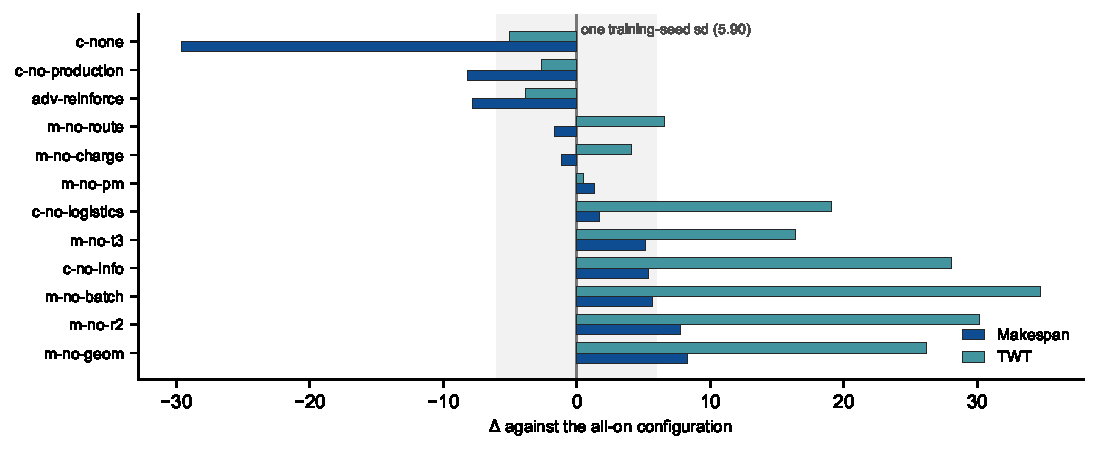
\includegraphics[width=\textwidth]{fig_ablation.pdf}
\caption{Ablation against the all-on configuration, the same numbers as
Table~\ref{tab:ablation}. The shaded band is one training-seed standard
deviation. The tardiness differences mostly fall outside it; the makespan
differences mostly do not.}
\label{fig:ablation}
\end{figure*}

Table~\ref{tab:ablation}, plotted in Figure~\ref{fig:ablation}, reads as two
groups.

Among the mechanism arms, the separation is between the mechanisms the
instance can exercise and the mechanisms it cannot. Three of them have nothing
to act on here: the charging constraint never activates under these parameters,
the maintenance interval is never reached on this instance, and congestion does
not bind at the reference load. Their makespan differences straddle zero
($-1.6$ to $+1.3$) and their tardiness differences are small ($+0.5$ to
$+6.6$), which is what a correctly implemented mechanism with no effect to make
should look like. The four mechanisms that do have something to act on --- the
aisle-segment tokens, the distance bias, the batch head, and the budget
mechanism --- have positive differences in every case: $+5.1$ to $+8.3$ in
makespan and $+16$ to $+35$ in tardiness. The grouping is not chosen after the
fact. Whether a mechanism can act is established independently of this table,
by measuring the constraint rather than the policy
(Tables~\ref{tab:active} and~\ref{tab:batching}).

What the table does not support is an ordering among the mechanisms. With one
training seed per arm, and a measured training-seed standard deviation of
5.90, the differences are of the same order as the seed-to-seed variation, and
a re-run with other seeds would shuffle the order. A single seed cannot
separate a mechanism that helps by five makespan units from a mechanism that
does nothing. The $p$ values in the table test consistency across five
\emph{evaluation} seeds, which is a different source of variation and does not
cover the training seed. We therefore report the grouping and not the ordering,
and Section~\ref{sec:conclusion} states how many seeds an ordering would need.
The three negative arms among the constraint groups --- production, all-off,
and the REINFORCE advantage --- fall inside the range that changing the
training seed alone can produce.

One further caveat applies to the three constraint-group arms. Switching off a
dynamics constraint changes the problem: the reference makespan moves from
109.05 to 117.77 when age-dependent failure is off and to 115.13 when multi-drop
travel is off. The absolute makespans of those arms are therefore not
comparable to the all-on configuration, and only the paired differences above
are meaningful.

The levels behind those differences are worth stating, because the differences
are differences of small numbers. Across the thirteen arms the total energy
account spans $0.0772$ to $0.0832$ kWh per minute of makespan, a range of
7.6\% of its mean, while the net account spans four times as much; machine
utilization ranges from $0.399$ to $0.704$, and the highest value belongs to
the all-off arm, which finishes ten jobs quickly because it faces the easiest
problem.



\subsection{What the benchmark actually exercises}
\label{sec:results:active}

A constraint that is modelled but never triggered contributes nothing to the
problem, and whether a constraint triggers is an empirical question. It can be
answered without training: run the reference schedule and count the events.
This measurement is a property of the constraint under the reference schedule,
not a property of any learned policy, so we report it for all ten instances of
the benchmark even though every policy result in this paper comes from MK01.

\begin{table}[htbp]
\centering
\caption{Constraint activation under the reference schedule, tier B switches,
one seed. Counts are per episode. The maintenance clock column gives the
largest accumulated spindle time reached by any machine, against a maintenance
interval of 120 minutes.}
\label{tab:active}
\setlength{\tabcolsep}{2.5pt}
\begin{threeparttable}
\begin{tabular}{@{}lrrrrr@{}}
\toprule
Instance & $C_{\max}$ & Failures & Forced PM & Max clock & Drained \\
\midrule
mk01 & 109.05 & 0 & \textbf{0} & \textbf{82} & 0 \\
mk02 & 74.72 & 0 & \textbf{0} & \textbf{45} & 0 \\
mk03 & 406.35 & 1 & 3 & 125 & 0 \\
mk04 & 270.75 & 0 & 1 & 122 & 0 \\
mk05 & 351.91 & 1 & 4 & 126 & 0 \\
mk06 & 233.77 & 1 & \textbf{0} & \textbf{105} & 0 \\
mk07 & 309.72 & 0 & 3 & 128 & 0 \\
mk08 & 777.85 & 5 & 16 & 133 & 0 \\
mk09 & 616.91 & 1 & 14 & 129 & 0 \\
mk10 & 501.02 & 1 & 9 & 128 & 0 \\
\bottomrule
\end{tabular}
\begin{tablenotes}\footnotesize
\item No vehicle ever drains on any instance, so the charging constraint is
      inert throughout the benchmark under the standard parameters. The
      maintenance constraint activates on seven of the ten instances; on the
      three marked in bold the accumulated spindle time stays below the
      interval, so no maintenance is ever forced. Vehicle failures occur 15 to
      114 times per episode depending on the instance and are not tabulated
      here.
\end{tablenotes}
\end{threeparttable}
\end{table}

Two consequences run through the rest of the paper. First, the charging
mechanism has nothing to act on: the fleet consumes 0.51--4.62 \kWh{} per
episode against a 2--4 \kWh{} battery, a factor of three to ten of headroom, so
the state never arises. Second, the maintenance mechanism has nothing to act on
in MK01 specifically, which is the instance all policy results come from. Both
are reported as facts about the parameterization rather than as properties of
the mechanisms.

\subsubsection{Where congestion begins to bind}
\label{sec:results:load}

The congestion mechanism shows a zero in Table~\ref{tab:ablation} on MK01, and
it is worth establishing whether that belongs to the instance or to the
parameters. Table~\ref{tab:load} varies the travel load through the vehicle
speed and the supply through the fleet size, and records the time vehicles
spend waiting for an aisle segment as a share of the makespan per vehicle.

\begin{table}[htbp]
\centering
\caption{Aisle contention as a function of travel load and fleet size, under
the reference schedule with all ten constraints on. Entries are the total time
vehicles wait for an aisle segment, divided by the fleet size and by the
makespan, in per cent.}
\label{tab:load}
\setlength{\tabcolsep}{5pt}
\begin{threeparttable}
\begin{tabular}{@{}lrcc@{}}
\toprule
Instance & Vehicle speed (m/s) & 3 vehicles & 6 vehicles \\
\midrule
mk01 & 1.00 & 0.31 & 0.20 \\
mk01 & 0.50 & 0.51 & 0.65 \\
mk01 & 0.25 & 1.23 & 1.33 \\
mk01 & 0.10 & \textbf{18.13} & \textbf{10.41} \\
\midrule
mk10 & 1.00 & 0.13 & 0.12 \\
mk10 & 0.50 & 0.27 & 0.35 \\
mk10 & 0.25 & 0.97 & 0.90 \\
mk10 & 0.10 & \textbf{4.94} & \textbf{5.09} \\
\bottomrule
\end{tabular}
\begin{tablenotes}\footnotesize
\item The nominal speed is 0.5~m/s. With a single vehicle the entry is zero at
      every speed, since one vehicle cannot contend with itself.
\end{tablenotes}
\end{threeparttable}
\end{table}

Three things are readable. First, the single-vehicle column is identically
zero at every speed, which is a property of the metric rather than a finding:
it confirms that what is being measured is interaction between vehicles and not
travel time as such. Second, at the nominal speed a vehicle waits for an aisle
segment well under one per cent of the time, and adding vehicles does not
change that. Third, the transition to a contended regime is abrupt rather than
gradual: on MK01 the wait goes from 1.2\% at a quarter of the nominal speed to
18\% at a tenth of it, and on MK10 from 1.0\% to 4.9\%. The constraint is
therefore not inert in general. It is inert at the benchmark's operating point,
where vehicle utilisation lies between 4\% and 23\%, and that is the sense in
which its zero in Table~\ref{tab:ablation} should be read.

\subsubsection{Batching opportunities}
\label{sec:results:batching}

The multi-drop travel model and its batching head were added because the load
capacity of a vehicle was a parameter the model carried but never used.
Whether the mechanism has anything to do depends on how often a pick-up point
holds more than one waiting task. Table~\ref{tab:batching} measures that
across the three instance sizes, again under the reference schedule.

\begin{table}[htbp]
\centering
\caption{Batching opportunities under the reference schedule. ``Pick-ups'' is
the number of times a vehicle collects at a pick-up point; the middle column
counts how often more than one task was available there.}
\label{tab:batching}
\setlength{\tabcolsep}{4pt}
\begin{threeparttable}
\begin{tabular}{@{}lrrrr@{}}
\toprule
Instance & Seed & Pick-ups & Multi-task & Mean per trip \\
\midrule
mk01 & 0 & 70 & 1 (1.4\%) & 1.014 \\
mk01 & 1 & 67 & 1 (1.5\%) & 1.015 \\
mk07 & 0 & 119 & 3 (2.5\%) & 1.042 \\
mk07 & 1 & 120 & 2 (1.7\%) & 1.033 \\
mk10 & 0 & 235 & 29 (12.3\%) & 1.140 \\
mk10 & 1 & 227 & 34 (15.0\%) & 1.163 \\
\bottomrule
\end{tabular}
\begin{tablenotes}\footnotesize
\item The maximum batch size reached is two on MK01 and three on MK07 and
      MK10. Under a first-in-first-out travel rule, which collects more
      aggressively, the rates rise to 3 of 64 pick-ups on MK01, 13 of 99 on
      MK07, and 55 of 204 on MK10.
\end{tablenotes}
\end{threeparttable}
\end{table}

MK01, the only instance on which policies are trained here, is the instance
with the fewest batching opportunities: 1.4\% of pick-ups against 12.3\% on
MK10. A mechanism that only acts when a batch can be formed will therefore
appear inert on MK01 for a reason that belongs to the instance. The
\texttt{m-no-batch} row of Table~\ref{tab:ablation} should be read with that in
mind, and it should not be read as a verdict on batching.

\subsection{Advantage ablation}
\label{sec:results:advantage}

This is the one experiment in the paper with five training seeds per arm,
because its conclusion is about the training procedure itself.
Table~\ref{tab:advantage} reports it.

\begin{table}[htbp]
\centering
\caption{Advantage ablation, five training seeds per arm, budget mechanism off,
all other switches identical. $p$ values are paired $t$-tests over the five
training seeds.}
\label{tab:advantage}
\setlength{\tabcolsep}{4pt}
\begin{threeparttable}
\begin{tabular}{@{}lrrr@{}}
\toprule
 & \texttt{scalar} & \texttt{reinforce} & \texttt{raw} \\
 & $(r-\bar r)/\sigma$ & $r - \bar r$ & $r$ \\
\midrule
Seed 0 & 84.04 & 71.12 & 84.97 \\
Seed 1 & 81.24 & 79.96 & 87.98 \\
Seed 2 & 87.19 & 75.31 & 90.72 \\
Seed 3 & 79.27 & 71.79 & 79.35 \\
Seed 4 & 71.56 & 85.85 & 85.41 \\
\midrule
Mean makespan & $80.66 \pm 5.90$ & $76.81 \pm 6.15$ & $85.69 \pm 4.22$ \\
Mean energy & 6.315 & 6.053 & 6.650 \\
Mean \TWT & 17.10 & 16.94 & 40.14 \\
\bottomrule
\end{tabular}
\begin{tablenotes}\footnotesize
\item Paired differences, makespan: \texttt{reinforce} $-$ \texttt{scalar}
      $= -3.85$ ($p = 0.48$); \texttt{raw} $-$ \texttt{scalar} $= +5.03$
      ($p = 0.11$); \texttt{raw} $-$ \texttt{reinforce} $= +8.88$
      ($p = 0.034$). Nine paired tests are reported in this section; a
      Bonferroni threshold over them is $0.0056$, which none of these reaches.
\end{tablenotes}
\end{threeparttable}
\end{table}

\begin{figure}[htbp]
\centering
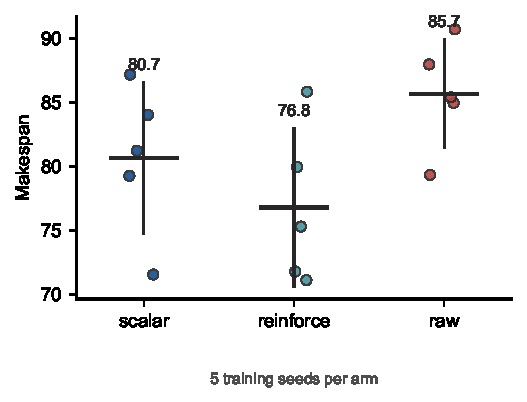
\includegraphics[width=\columnwidth]{fig_advantage.pdf}
\caption{Advantage ablation, five training seeds per arm. Points are individual
seeds; the horizontal bar is the arm mean and the vertical bar is one standard
deviation. The three arms are identical in every switch and hyperparameter;
only the advantage differs.}
\label{fig:advantage}
\end{figure}

Figure~\ref{fig:advantage} gives two findings.

Subtracting a group-mean baseline has an effect. The arm that uses the raw
reward, with no baseline subtracted, is worse than the arm that subtracts the
group mean by 8.88 makespan units, with four of five seeds agreeing on the
sign. The uncorrected $p$ value is 0.034; with nine paired tests in this
section, the Bonferroni threshold is 0.0056, so we report this as a consistent
direction rather than as a significant effect.

Dividing by the group standard deviation has no measurable effect. The
\texttt{scalar} and \texttt{reinforce} arms differ by 3.85 makespan units with
$p = 0.48$, and the per-seed differences change sign. On this problem the
normalization step of the group-relative advantage is not doing detectable
work; the baseline subtraction is.

This distinction matters for how the method is described. The usual statement
is that group-relative advantages are necessary. What the data support is
narrower: a group-mean baseline is necessary, and the division by the group
standard deviation is not measurably different from omitting it.

This table is also where the seed variance was measured, and it is the reason
the rest of this paper's ablations are labelled as they are. The per-arm
standard deviation is 4--6 makespan units; the differences between arms are
4--9. Before this experiment was run, a single-seed comparison of the
\texttt{scalar} and \texttt{reinforce} arms read as a 15.4\% win for
\texttt{reinforce}; with five seeds it is 4.8\% with $p=0.48$. The
\texttt{scalar} arm's own seed 4 (71.56) is lower than the
\texttt{reinforce} arm's seed 0 (71.12) for all practical purposes.

\subsection{The objectives}
\label{sec:results:front}

Table~\ref{tab:front} reports five preference vectors trained to completion,
plus the default weight vector derived from the reference schedule.

\begin{table}[htbp]
\centering
\caption{Preference sweep on tier B. The three
one-hot vertices were trained as the single-objective baseline arms of
Table~\ref{tab:main}. ``Non-dominated'' is over the six rows of this table.}
\label{tab:front}
\setlength{\tabcolsep}{4pt}
\begin{threeparttable}
\begin{tabular}{@{}lrrrr@{}}
\toprule
Point & Preferences & Makespan & Energy & \TWT \\
\midrule
\texttt{b-ms} & $(1,0,0)$ & \textbf{74.09} & \textbf{5.790} & 5.977 \\
\texttt{b-twt} & $(0,0,1)$ & 77.30 & 6.048 & 7.392 \\
\texttt{e-me} & $(0.5,0.5,0)$ & 77.27 & 6.053 & 9.594 \\
\texttt{full} & $w$-derived & 78.90 & 6.160 & \textbf{5.042} \\
\texttt{e-eq} & $(1/3,1/3,1/3)$ & 80.96 & 6.333 & 20.456 \\
\texttt{b-en} & $(0,1,0)$ & 96.93 & 7.434 & 97.458 \\
\bottomrule
\end{tabular}
\begin{tablenotes}\footnotesize
\item The default weight vector is $w = (0.062, 0.819, 0.120)$, derived from the
      reference schedule. ``Non-dominated'' marks \texttt{b-ms} and
      \texttt{full}. All six runs completed all ten jobs with no horizon
      truncation.
\end{tablenotes}
\end{threeparttable}
\end{table}

The attainable front collapses to two points: \texttt{b-ms} and \texttt{full}.
The three remaining preference vectors, including both interior points, are
dominated.

The collapse is a property of the objectives, not of the search. On this
instance the three objectives are strongly aligned: a policy that does well on
makespan also does well on energy and tardiness. The makespan-only arm is not
merely non-dominated; it is within 0.9 tardiness units of the default arm while
being better on the other two objectives.

Two caveats. The endpoint of a single training run moves: the
\texttt{e-me} arm read 72.65 / 5.683 / 3.038 at step 270, which would have
dominated every point in the table, and 77.27 / 6.053 / 9.594 at step 300. Five
evaluation seeds do not pin the endpoint of a single arm. And the effective
strength of the budget mechanism differs between preference arms, because the
penalty enters before group normalization and is therefore scaled by the group
reward spread; the arms in Table~\ref{tab:front} differ in both the preference
vector and the effective penalty strength.

\subsubsection{The energy account and the makespan}
\label{sec:results:energy}

The paper reports energy as a third objective, and one property of the account
has to be stated so that the energy column is not read as something it is not.
Total energy as defined by Equation~\eqref{eq:energy} is close to
rank-equivalent with the makespan: across the thirteen ablation runs the ratio
of the two spans 7.6\%, and their rank correlation is $\rho = 0.978$.

The reason is not a finding but a consequence of the definition. Machine
processing accounts for 38--45\% of the total, machine standby for 21--31\%,
machine setup for 13--17\%, vehicles for 8--9\%, and the fixed shop load for
8.5\%; of these, the fixed shop load is charged over the makespan explicitly,
vehicle standby is likewise horizon-bound, and machine standby is not merely
correlated with the makespan but determined by it, since the time a machine
spends idle is the horizon minus the time it spends working. Together these
terms are a little under half of the total, and they are affine in the makespan
for any schedule whatsoever. The aggregate account therefore cannot move
independently of the makespan by more than the variation in the remaining
terms, and a schedule cannot be made more energy-efficient under this account
without also being made shorter. A net account that keeps only the terms
attributable to work actually performed, and drops the three horizon-bound
ones, is not tied to the makespan in this way ($\rho = 0.582$); it is reported
in Equation~\eqref{eq:energy:net} and used in Section~\ref{sec:results:front},
but the reward is trained on the total account, so it is a reading and not an
objective here.

Two consequences for reading the tables. The energy column of
Table~\ref{tab:main} should be read as a restatement of the makespan rather
than as an independent axis: under the standard account the reported
three-objective problem has an effective dimension of two. And the same is true
of the published work this paper compares against indirectly, because the
account is the standard one; the point is about the account, not about any
particular study. Section~\ref{sec:conclusion} records what would be needed to
turn the net account into an objective.

A counterfactual bounds the sensitivity to one modelling choice. The machine
standby power is taken from the loaded-idle column of the cited source rather
than its separately tabulated standby power; replacing it with the lower
tabulated value reduces the mean total energy by 12.9\% and widens the ratio
spread from 7.6\% to 16.6\%, while leaving the rank correlation unchanged at
$\rho = 0.973$. The choice moves the level of the reported energy, not its
ordering.

\subsubsection{Sensitivity to the assumed parameters}
\label{sec:results:sensitivity}

Most constraint parameters have no published source, and the sensitivity of the
reported results to them is part of what the paper has to establish.
Table~\ref{tab:sens} re-evaluates the tier B policy under perturbed dynamics.

\begin{table*}[htbp]
\centering
\caption{Sensitivity of the tier B policy to the assumed parameters, five
evaluation seeds. The policy is held fixed and only the dynamics change. The
default column repeats the tier B row of Table~\ref{tab:main}. Values are
makespan / energy / \TWT.}
\label{tab:sens}
\setlength{\tabcolsep}{5pt}
\begin{threeparttable}
\small
\begin{tabular}{@{}lrrr@{}}
\toprule
Parameter & Low & Default & High \\
\midrule
Setup time (min) & 1.0 & 2.0 & 4.0 \\
\quad & 67.38 / 5.359 / 0.00 & 78.90 / 6.160 / 5.04 & 95.73 / 7.315 / 100.07 \\
Failure rate & $\times 0.5$ & $\times 1$ & $\times 2$ \\
\quad & 78.81 / 6.152 / 4.89 & 78.90 / 6.160 / 5.04 & 84.74 / 6.593 / 45.41 \\
Rework probability & 0.025 & 0.05 & 0.10 \\
\quad & 73.53 / 5.773 / 3.11 & 78.90 / 6.160 / 5.04 & 81.99 / 6.399 / 8.05 \\
Maintenance interval (min) & 240 & 120 & 60 \\
\quad & \multicolumn{3}{c}{bit-identical to default at 240} \\
\quad & --- & 78.90 / 6.160 / 5.04 & 79.90 / 6.229 / 5.04 \\
Vehicle MTBF (min) & 240 & 480 & 960 \\
\quad & 80.02 / 6.240 / 7.73 & 78.90 / 6.160 / 5.04 & 78.81 / 6.154 / 5.16 \\
\bottomrule
\end{tabular}
\begin{tablenotes}\footnotesize
\item Job weights are not swept: the evaluation path hard-codes equal weights,
      so the parameter has no entry point. Re-evaluation holds the policy and
      its normalization context fixed and changes only the dynamics. The
      maintenance row is identical at 240 because MK01 never reaches the
      default interval in the first place.
\end{tablenotes}
\end{threeparttable}
\end{table*}

\begin{figure}[htbp]
\centering
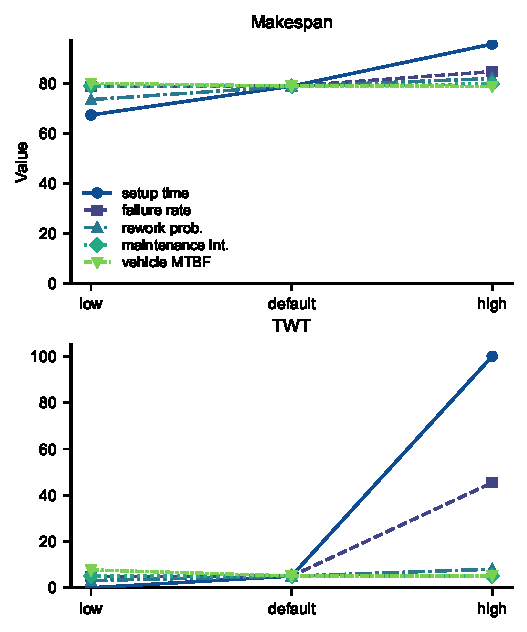
\includegraphics[width=\columnwidth]{fig_sensitivity.pdf}
\caption{Sensitivity to the assumed parameters, the same numbers as
Table~\ref{tab:sens}. The policy is held fixed and only the dynamics change.
Parameter levels are not commensurate, so the horizontal axis is the level
index rather than a physical value, and each curve is identified by marker and
line style as well as by colour. The setup time and the failure rate dominate
the makespan; the tardiness panel separates the parameters far more sharply,
and the maintenance interval is flat on both because the instance never
reaches it.}
\label{fig:sensitivity}
\end{figure}

The two largest levers, in Figure~\ref{fig:sensitivity}, are the setup time and
the machine failure rate. Over
the swept range the setup time moves the makespan by 28 points and the
tardiness by 100, and the failure rate by 5.8 and 40. Rework is intermediate,
at 8.5 and 5. Vehicle failure and the maintenance interval move little, and the
maintenance parameter at 240 is bit-identical to the default because the
instance never reaches the interval at either setting.

Re-evaluation approximates retraining for these parameters. We trained two
fresh policies in the perturbed environment, at the most adverse level of each
of the two largest levers. For the setup time the retrained policy reaches
102.85 against 95.73 for the re-evaluated one; for the failure rate, 82.91
against 84.74. Both gaps are of the same order as the training-seed standard
deviation of 5.90 for makespan, so the order the re-evaluation reports is
informative. Tardiness moves much further, by $+18.1$ and $-24.5$, and the
re-evaluated tardiness should not be read as a retrained value.

\subsection{Discussion}
\label{sec:discussion}

The two tiers say more together than either says alone. On tier B, where the
ten constraints are present, the learned policy dominates every out-of-sample
point of the NSGA-II front and beats the rule baseline by 26.5 in makespan. On
tier A, where the constraints are switched off and the problem is easy, the
ordering reverses and the metaheuristic edges ahead. That pair locates the
policy's advantage in its representation of the constrained state rather than
in its search behaviour, which is the claim this paper set out to test.

The advantage ablation narrows a claim that is often stated too broadly. A
group-mean baseline is doing measurable work; the division by the group
standard deviation is not measurably different from omitting it. That is a
statement about the training procedure and not about this problem in
particular, and it is the one comparison in the paper that rests on enough
training seeds to be read as an estimate rather than as a measurement.

The constraint results are consistent rather than surprising. Every mechanism
that the instance can exercise shows a positive difference when it is removed,
and every mechanism that it cannot exercise sits at zero; the two groups are
separated by properties of the constraint that were measured independently of
the policy. What the ablation does not support is an ordering among the
mechanisms, and the reason is sample size rather than effect size.


\section{Conclusion}
\label{sec:conclusion}

This paper studied production--logistics collaborative scheduling with ten
modelled constraints and three reported objectives, using a joint-chain
formulation in which all production and logistics decisions of an episode form
a single decision chain trained by group-relative policy optimization. The
policy's parts are standard, a Transformer encoder with candidate-scoring
heads; what the paper contributes is the chain that joins the two decision
layers, the encoding that puts the aisle network into the state, and the
measurement of what the ten constraints do when they are all present.

The method beats a rule baseline by 26.5 in makespan on the fully constrained
problem and dominates every out-of-sample point of an NSGA-II front, while
losing narrowly to the same metaheuristic on the unconstrained problem. That
combination locates the method's advantage in its representation of the
constrained state rather than in its search behaviour. On the objective side,
the aggregate energy consumption commonly reported in this literature is close
to rank-equivalent with the makespan, because the terms that dominate it are
linear in the horizon by construction; under that account the reported
three-objective problem has an effective dimension of two, which is consistent
with the observed collapse of the preference front to two points. A net account
that removes the horizon-linear terms restores independent ordering.

\paragraph{Limitations} The evaluation is a first pass and the scope is narrow.
Every number comes from a single instance of the benchmark, and MK01 is the
instance least favourable to the batching mechanism, so the batching results
here are not a verdict on batching. Except for the advantage ablation, each
configuration was trained once. Against that, the training-seed standard
deviation is measured rather than assumed: it is 5.90 makespan units on the same
configuration, which is the order of most of the differences we report, and it
is why the ablation table is presented without a ranking.

The comparison uses a rule, a single-objective version of our own method, and
NSGA-II. It does not use a published deep reinforcement learning method, which
is the baseline a reviewer would most reasonably ask for; adapting one to this
simulation is substantial work, and Section~\ref{sec:related:incomparable}
explains the boundary conditions under which any such number could be compared.
A state-of-the-art metaheuristic for the flexible job shop is absent for the
same reason. On the constraint side, two of the ten do not activate under the
reported parameters: the charging constraint never fires across the benchmark,
and maintenance does not trigger on MK01, so the budget mechanism penalizes four
constraints in practice rather than the six it is configured with. The
consequence is stated plainly: this paper reports no evidence on whether the
charging mechanism works, and establishes that only in a configuration where
vehicles actually drain. Most of the constraint parameters have no published
source and are values we chose; the sensitivity analysis in
Section~\ref{sec:results:sensitivity} reports how far the results move when they
change, but does not make them cited. One parameterization of the reported
energy is conservative: the machine standby power is taken from the loaded-idle
column of the cited source rather than its separately tabulated standby power,
which overstates standby energy by 12.9\% of the total without changing any
ordering. Finally, the paper proves no bound and no convergence guarantee.

\paragraph{Future work} Three measurements would change the conclusions rather
than extend them. The ablation table reports a grouping, not an ordering,
because one training seed per arm cannot separate differences of the size it
reports. An ordering would need about ten seeds per arm, some hundred and fifty
runs at the cost measured in Section~\ref{sec:method:cost}, with the number set
by the smallest difference the table is meant to resolve: at a seed-to-seed
spread of eight makespan units, an effect of eight units needs eight seeds and
an effect of five needs twenty. The comparison against the baselines is much
cheaper to settle, because its effect is three times the seed-to-seed spread;
three seeds per arm would certify it. Running the mechanisms on further
instances of the benchmark would separate the effects that belong to the
mechanism from those that belong to MK01, which matters most for batching and
for maintenance. And training with the net energy account as the reward, rather
than measuring it after the fact, would test whether the third dimension
available at the measurement level is usable at the optimization level. The
comparison against a published deep reinforcement learning method remains the
piece of work this paper most needs done next.


% 清空所有未决浮动体——否则 table*/figure* 会漂到参考文献之后。
\clearpage

\bibliographystyle{elsarticle-num}
\bibliography{refs}

\end{document}
